\chapter{Cinématique des robots manipulateurs II: Le mouvement}
\label{sec:cinediff}



Dans le chapitre \ref{sec:cine1}, les méthodes pour modéliser la position, l'orientation ont été présentée. Ce chapitre présente les méthodes associés pour représenter leurs variation dans le temps, c'est-à-dire la vitesse. Les premières sections décrivent les principes généraux et ensuite des méthodes spécifiques pour les robots manipulateurs sont présentées. 

%Chapitre en construction!


%%%%%%%%%%%%%%%%%%%%%%%%%%%%%%%%%%%%%%%%%%%%%%%%%%%%%%%%%%%%%%
\section{Référentiel} 
%%%%%%%%%%%%%%%%%%%%%%%%%%%%%%%%%%%%%%%%%%%%%%%%%%%%%%%%%%%%%%

Un référentiel est un solide ou un ensemble de points par rapport auquel un observateur qui mesure un mouvement est fixe. Une position ou un mouvement ne peut être défini par rapport au vide et il n'y a pas de référentiel absolu, le choix du référentiel est donc un choix arbitraire de point de vue. Il est à noter que \textbf{contrairement au choix d'un repère, le choix du référentiel influence "la physique" du problème}, par exemple l'énergie cinétique d'un objet n'est pas la même selon le référentiel alors que cette quantité est indépendante du système de coordonnées. Un référentiel dit inertiel ou Galiléen (vitesse et orientation constante) est préférable si on souhaite éventuellement appliquer les équations de Newtons, car des facteurs correctifs (ex.: la force centrifuge) doivent être ajoutés aux équations dynamiques si un référentiel non-inertiel est utilisé. La notion de référentiel est critique pour le calcul de vitesses et accélérations, mais on peut en faire abstraction pour les problèmes de cinématique et statique qui n'impliquent pas la notion d'évolution dans le temps. 


%%%%%%%%%%%%%%%%%%%%%%%%%%%%%%%%%%%%%
\subsection{Référentiel vs. repère}
Pour décrire le mouvement d'un objet, les concepts de référentiel, origine et base vectorielle sont important à distinguer. En quelques mots, un \textbf{référentiel} est un point de vue utilisé pour décrire un phénomène, une \textbf{origine} c'est un point par rapport auquel les mesures de position sont faites et une \textbf{base} vectorielle représente l'orientation du système d'axe utilisé. Ces trois éléments peuvent être choisi indépendamment.  Ensuite, un \textbf{repère} c'est la combinaison d'une base et d'une origine. Par exemple, pour décrire la position d'un bateau, typiquement le référentiel utilisé serait la Terre, l'origine des mesures de position pourrait être le port le plus près, et la base pour exprimer cette position serait le système d'axe nord-sud/est-ouest. Il est important de noter que tous ces choix sont indépendants et les confondre est une source d'erreur courante en cinématique. Le reste de cette section discute de ce qui les distingue.

\video{Référentiel vs. repère vs. base vectorielle}{https://youtu.be/Uv_MbbfkiS4}

%%%%%%%%%%%%%%%%%%%%%%%%%%%%%%%%%%%%%%%%%%%%%%%%%%%%%%%%%%%%%%%%%%%%%%%%%%%%%
\begin{figure}[H]
	\centering
		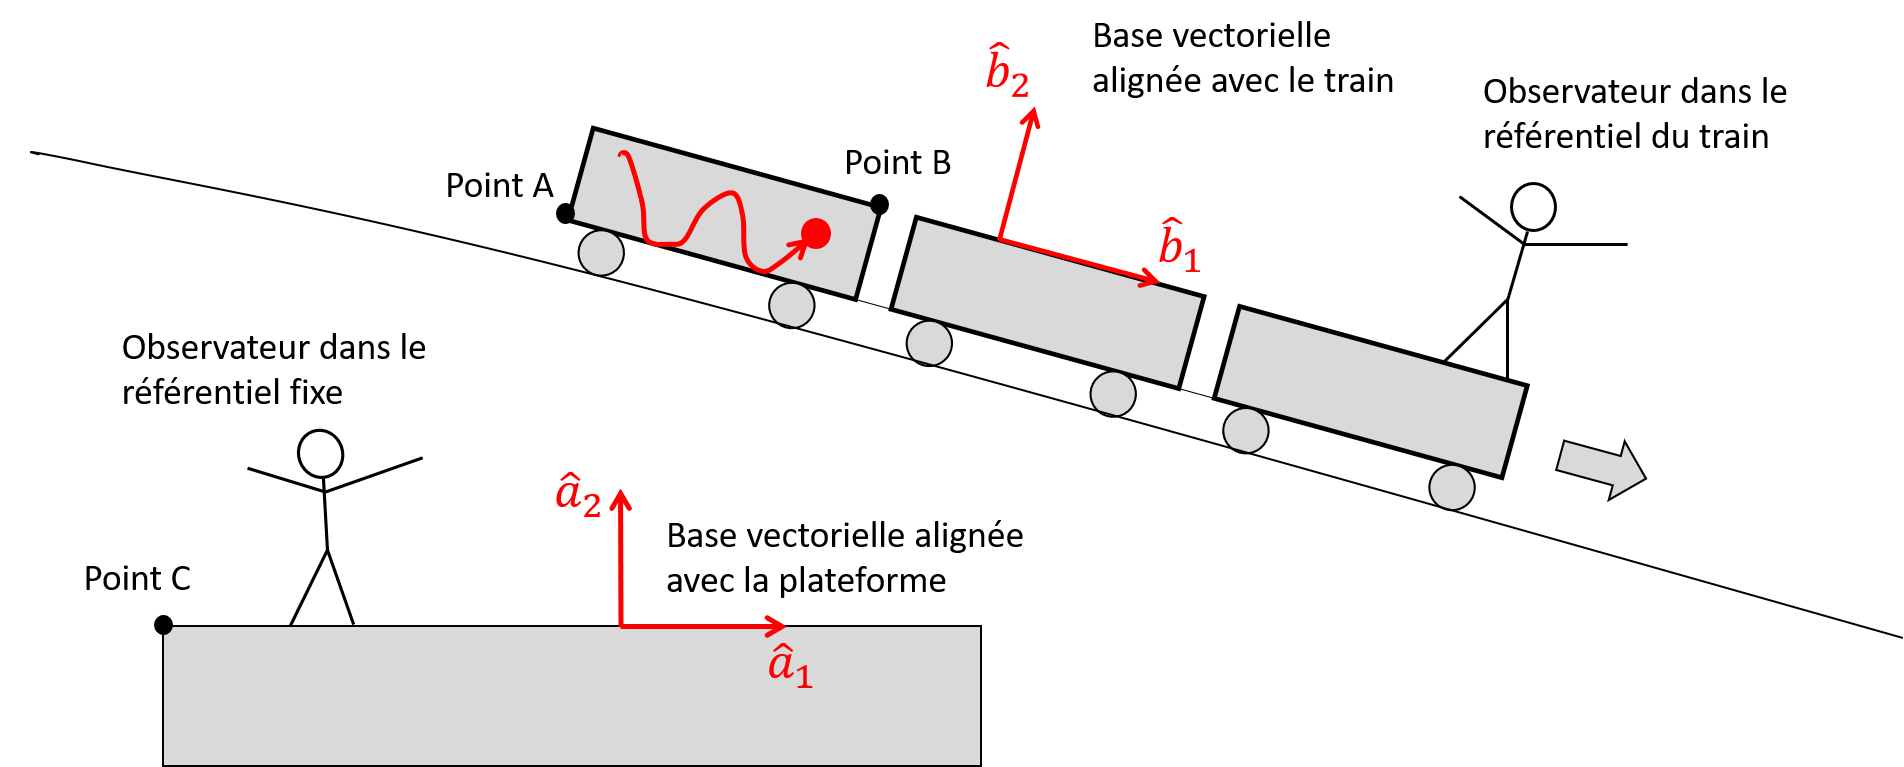
\includegraphics[width=0.90\textwidth]{train.png}
	\caption{Exemple de référentiels, points d'origine et bases vectorielles}
	\label{fig:train}
\end{figure}
%%%%%%%%%%%%%%%%%%%%%%%%%%%%%%%%%%%%%%%%%%%%%%%%%%%%%%%%%%%%%%%%%%%%%%%%%%%%%%%

La figure \ref{fig:train} illustre ces concepts par un exemple où un train descend une pente à vitesse constante et un ballon rebondit sur le sol du troisième wagon. Deux bases vectorielles sont définies, une alignée avec l'horizontale et une alignée avec le train. Plusieurs points d'origine pour les mesures de position sont aussi disponibles. Finalement, deux référentiels sont définis, un référentiel attaché à la Terre (fixe) et un référentiel qui est attaché au train. Les coordonnées d'un vecteur-colonne qui décris la position du ballon:
%%%%%%%%%%%%%%%%%%%%%%%%%%%%%%%%%%%%%
\begin{equation}
\col{r}_{Ball} = \left[ \begin{array}{c} r_1 \\ r_2 \end{array} \right]
\end{equation}
%%%%%%%%%%%%%%%%%%%%%%%%%%%%%%%%%%%%%
sont illustrés pour différents choix d'origine et de base vectorielle, lorsque que le référentiel fixe est utilisé (figure \ref{fig:refex1}) et lorsque que le référentiel du train est utilisé (figure \ref{fig:refex2}). Il est à noter que les points d'origine sont ici fixés à la Terre lorsque le référentiel fixe est utilisé, et fixés au train lorsque que le référentiel du train est utilisé. Comme illustré pour cet exemple, \textbf{un changement d'origine est analogue à une translation} de la trajectoire, \textbf{un changement de base vectorielle est analogue à une rotation} de la trajectoire, et \textbf{un changement de référentiel est ici analogue à une dilatation} de la trajectoire dans la direction $\hat{b}_1$, qui correspond à la direction de la vitesse du train. 

%%%%%%%%%%%%%%%%%%%%%%%%%%%%%%%%%%%%%%%%%%%%%%%%%%%%%%%%%%%%%%%
\begin{figure}[p]
				%\vspace{-10pt}
        \centering
        \subfloat[Repère $\{ A, \hat{a}_1, \hat{a}_2, \hat{a}_3\}$]{
				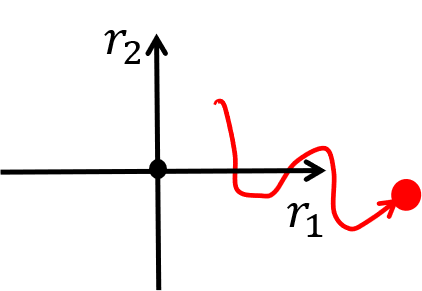
\includegraphics[width=0.23\textwidth]{ref_fixe_r_a_A.png}
				} \hspace{20pt}
				\subfloat[Repère $\{ B, \hat{a}_1, \hat{a}_2, \hat{a}_3\}$]{
				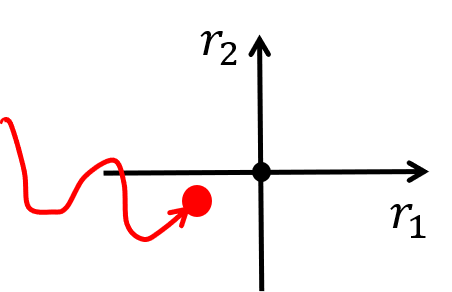
\includegraphics[width=0.24\textwidth]{ref_fixe_r_a_B.png}
				} \hspace{190pt}
				\subfloat[Repère $\{ A, \hat{b}_1, \hat{b}_2, \hat{b}_3\}$]{
				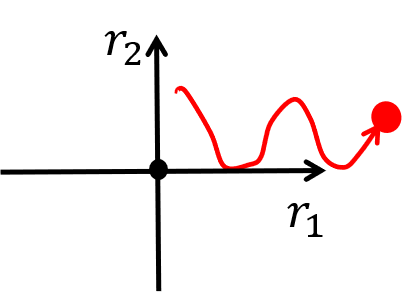
\includegraphics[width=0.22\textwidth]{ref_fixe_r_b_A.png}
				} \hspace{20pt}
				\subfloat[Repère $\{ B, \hat{b}_1, \hat{b}_2, \hat{b}_3\}$]{
				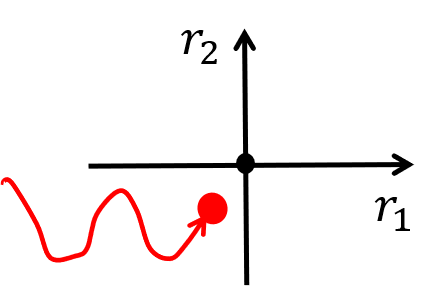
\includegraphics[width=0.24\textwidth]{ref_fixe_r_b_B.png}
				}
        \caption{Trajectoire du ballon avec un repère attaché au \textbf{référentiel fixe}}
				\label{fig:refex1}
\end{figure}
%%%%%%%%%%%%%%%%%%%%%%%%%%%%%%%%%%%%%%%%%%%%%%%%%%%%%%%%%%%%%%%%%

%%%%%%%%%%%%%%%%%%%%%%%%%%%%%%%%%%%%%%%%%%%%%%%%%%%%%%%%%%%%%%%
\begin{figure}[p]
				%\vspace{-10pt}
        \centering
				\subfloat[Repère $\{ A, \hat{a}_1, \hat{a}_2, \hat{a}_3\}$]{
				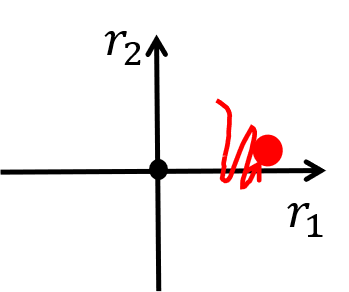
\includegraphics[width=0.22\textwidth]{ref_train_r_a_A.png}
				} \hspace{20pt}
				\subfloat[Repère $\{ B, \hat{a}_1, \hat{a}_2, \hat{a}_3\}$]{
				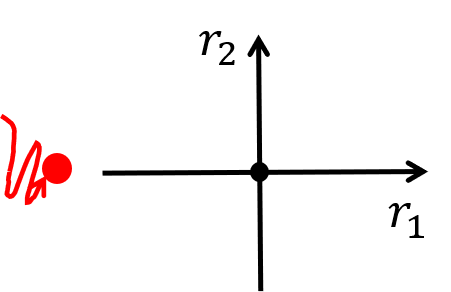
\includegraphics[width=0.25\textwidth]{ref_train_r_a_B.png}
				} \hspace{190pt}
				\subfloat[Repère $\{ A, \hat{b}_1, \hat{b}_2, \hat{b}_3\}$]{
				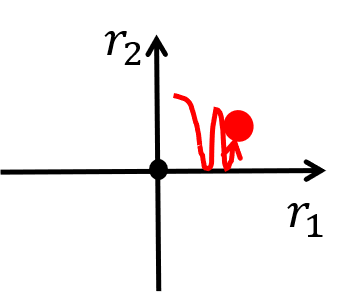
\includegraphics[width=0.22\textwidth]{ref_train_r_b_A.png}
				} \hspace{20pt}
				\subfloat[Repère $\{ B, \hat{b}_1, \hat{b}_2, \hat{b}_3\}$]{
				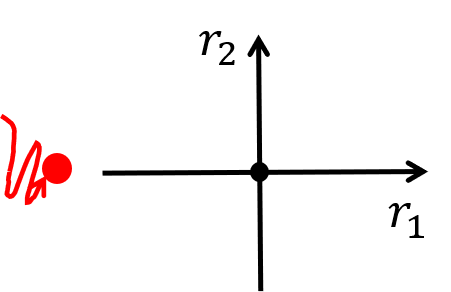
\includegraphics[width=0.25\textwidth]{ref_train_r_a_B.png}
				}
        \caption{Trajectoire du ballon avec un repère attaché au \textbf{référentiel du train}}
				\label{fig:refex2}
\end{figure}
%%%%%%%%%%%%%%%%%%%%%%%%%%%%%%%%%%%%%%%%%%%%%%%%%%%%%%%%%%%%%%%%%





%%%%%%%%%%%%%%%%%%%%%%%%%%%%%%%%%%%%%%%%%%%%%%%%%%%%%%%%%%%%%%
\newpage
\section{Vitesse et dérivée d'un vecteur position} 
%%%%%%%%%%%%%%%%%%%%%%%%%%%%%%%%%%%%%%%%%%%%%%%%%%%%%%%%%%%%%%

Un vecteur de vitesse est définit comme la dérivée temporelle d'une vecteur de position:
%%%%%%%%%%%%%%%%
\begin{equation}
\vec{v}_{B/A} = \frac{d}{dt} \vec{r}_{B/A}
\end{equation}
%%%%%%%%%%%%%%%
Toutefois, pour avoir la notion de vitesse précise qui correspond à un quantité de mouvement (momentum) qui peut être utilisée dans les divers lois de la physique (ex. conservation du mouvement, conservation de l'énergie, etc.), la dérivée doit être faite par rapport à un observateur Galiléen, aussi appelé un référentiel inertiel. Donc pour avoir la vitesse $\vec{v}_{B}$ d'un point $B$ il faut 1) que la dérivée soit faite par rapport à une base vectorielle avec un orientation fixe dans le référentiel Galiléen, et 2) que le vecteur position dérivé soit par rapport à un point d'origine fixe dans le référentiel Galiléen.
%%%%%%%%%%%%%%%%
\begin{equation}
\underbrace{
\vec{v}_{B}
}_{\text{ Vitesse du point B}}
= \underbrace{ 
\frac{d}{dt} 
}_{\text{observateur Galiléen}}
\vec{r}_{B/
\underbrace{A
}_{\text{Point fixe}}
}
\end{equation}
%%%%%%%%%%%%%%%
Avec cette définition, le vecteur vitesse est défini seulement par un seul point contrairement au vecteur position qui prend un sens seulement avec une origine.
La méthode la plus simple pour déterminer le vecteur vitesse d'un point basé sur une expression connue pour son vecteur position est d'exprimer le vecteur position dans un repère fixe, et ensuite de dériver chaque composante. Donc si il est possible d'exprimer le vecteur position d'un point $B$ par rapport à un point fixe $A$ et en utilisant une base vectorielle fixe $a$:
%%%%%%%%%%%%%%%%
\begin{equation}
\vec{r}_{B/A} = x \hat{a}_1 +  y \hat{a}_2 +  z \hat{a}_3
\end{equation}
%%%%%%%%%%%%%%%
il suffit de dériver l'expression de chaque composante dans cette base pour déterminer le vecteur vitesse du point $B$:
%%%%%%%%%%%%%%%%
\begin{equation}
\vec{v}_{B} = \frac{d}{dt} \vec{r}_{B/A} = 
\dot{x} \hat{a}_1 +  \dot{y} \hat{a}_2 +  \dot{z} \hat{a}_3
\end{equation}
%%%%%%%%%%%%%%%

%%%%%%%%%%%%%%%%%%%%%%%%%%%%%%%%%%%%%%%%%%%%%%%%%%%%%%%%%%%%%%%%%%%%%%%%%%%
\subsection{Dérivée d'un vecteur position exprimé avec une base mobile}
\label{sec:diffposmobilebase}

\note{Notation pour les repère fixes et mobiles}{ Pour les sections suivantes, les expressions sont développé en considérante que les repères notés $A$ (base $a$ et origine $A$) sont fixes dans le référentiel inertiel et que les repères notés $B$ (base $b$ et origine $B$) sont arbitraires donc potentiellement mobiles.}

Dans certaines situations, le vecteur position est plus naturellement exprimé dans un repère mobile, cette section développe des expressions qui peuvent être utilisée pour déterminer le vecteur vitesse sans avoir à tout transférer dans un repère inertiel. Si on connaît les composantes un vecteur position dans une base mobile $b$:
%%%%%%%%%%%%%%%%
\begin{equation}
\vec{r}_{B/A} = x \hat{b}_1 +  y \hat{b}_2 +  z \hat{b}_3
\end{equation}
%%%%%%%%%%%%%%%
Lorsqu'on dérive par rapport au temps, il faut tenir compte que les vecteurs unitaires de la base $b$ on une direction qui change dans le temps, et donc une dérivée temporelle non-nulle:
%%%%%%%%%%%%%%%%
\begin{align}
\vec{v}_{B} &= \frac{d}{dt} \vec{r}_{B/A} = 
\underbrace{
\dot{x} \hat{b}_1 +  \dot{y} \hat{b}_2 +  \dot{z} \hat{b}_3 
}_{ {}^{b}\frac{d}{dt} \vec{r}_{B/A}  }
+ 
\underbrace{
x \dot{\hat{b}}_1 +  y \dot{\hat{b}}_2 +  z \dot{\hat{b}}_3
}_{  \vec{w}_{b/a} \, \times \, \vec{r}_{B/A}  } 
\label{eq:speedvec}
\end{align}
%%%%%%%%%%%%%%%
Il y a donc deux sources de contribution au vecteur vitesse, le taux de variation des composantes et le taux de variation de la direction des vecteurs unitaires. La dérivée temporelle des vecteurs unitaires est directement reliée à la vitesse angulaire de la base $b$ (voir section \ref{sec:angularspeed}, et cette contribution peut être calculée avec le produit vectoriel d'un vecteur de vitesse angulaire de la base $b$ par rapport à une base fixe $a$ fois le vecteur de position:
%%%%%%%%%%%%%%%%
\begin{align}
\vec{v}_{B} &= 
\underbrace{
{}^{b}\frac{d}{dt} \vec{r}_{B/A} 
}_{\text{Observateur mobile}}
+  
\underbrace{
\vec{w}_{b/a} \, \times \, \vec{r}_{B/A}
}_{\text{Effet de la vitesse angulaire}}
\label{eq:speedprodvec}
\end{align}
%%%%%%%%%%%%%%%
où $b$ est une base mobile, $a$ est une base fixe dans le référentiel inertiel, le terme ${}^{b}\frac{d}{dt}$ représente le taux de variation vu par un observateur dans le référentiel non-inertiel qui tourne avec la base $b$ et $\vec{w}_{b/a}$ est la vitesse angulaire de la base $b$ p/r à une base $a$ inertielle.


\paragraph{Équation matricielle équivalente avec les composantes}:

On peut trouver une relation équivalente qui implique les vecteur-colonnes de composantes et les matrices de rotation. Le vecteur vitesse est la dérivée temporelle des composantes dans la base fixe $a$, on peut donc substituer par le vecteur-colonne de composantes dans la base $b$ fois la matrice de rotation ${}^{a}R^b$ et prendre la dérivée:
%%%%%%%%%%%%%%%%
\begin{align}
\col{v}_{B}^a &= \frac{d}{dt} \col{r}_{B/A}^a = 
\frac{d}{dt} \left( {}^{a}R^b \, \col{r}_{B/A}^b \right) 
\end{align}
%%%%%%%%%%%%%%%
Ici on applique la règle de dérivé d'un produit et comme avec la relation vectorielle de l'équation \eqref{eq:speedvec}, on trouve deux termes:
%%%%%%%%%%%%%%%%
\begin{align}
\col{v}_{B/A}^a &=
{}^{a}R^b \, \col{\dot{r}}_{B/A}^b + {}^{a}\dot{R}^b \, \col{r}_{B/A}^b 
\end{align}
%%%%%%%%%%%%%%%
Toutefois ici le taux de variation de la direction de la base mobile $b$ est représenté par la dérivée temporelle de la matrice de rotation ${}^{a}R^b$ (voir section \ref{sec:angularspeed}). On peut utiliser une expression qui utilise les composantes de la vitesse angulaire de la base $b$ pour déterminer la dérivée de la matrice de rotation
%%%%%%%%%%%%%%%%
\begin{align}
\col{v}_{B}^a &=
{}^{a}R^b \, \col{\dot{r}}_{B/A}^b + (\col{w}_{b/a}^a)^{\times} \, {}^{a}R^b \, \col{r}_{B/A}^b \\
\col{v}_{B}^a &=
{}^{a}R^b \, \col{\dot{r}}_{B/A}^b +  {}^{a}R^b \, (\col{w}_{b/a}^b)^{\times} \, \col{r}_{B/A}^b
\end{align}
%%%%%%%%%%%%%%%
pour obtenir une forme équivalente à l'expression vectorielle précédemment obtenue (eq. \eqref{eq:speedprodvec}, mais impliquant les vecteurs-colonnes de composantes et la matrice de rotation:
%%%%%%%%%%%%%%%%
\begin{align}
\vec{v}_{B} = {}^{b}\frac{d}{dt} \vec{r}_{B/A} +  \vec{w}_{b/a} \, \times \, \vec{r}_{B/A}
\quad \Leftrightarrow \quad 
\col{v}_{B}^{a} = {}^{a}R^b \left[ \col{\dot{r}}^b_{B/A} +  (\col{w}_{b/a}^b)^{\times} \col{r}^b_{B/A}  \right] 
\end{align}
%%%%%%%%%%%%%%%



%%%%%%%%%%%%%%%%%%%%%%%%%%%%%%%%%%%%%%%%%%%%%%%%%%%%%%%%
\newpage
\section{Vitesse angulaire et dérivée d'une matrice de rotation}
\label{sec:angularspeed}
%%%%%%%%%%%%%%%%%%%%%%%%%%%%%%%%%%%%%%%%%%%%%%%%%%%%%%%%

La représentation de l'orientation a plusieurs difficultés mathématiques: pour représenter seulement 3 DDL les matrices de rotation ont 9 paramètres, les rotation ne sont pas commutative, etc. Toutefois, les petites rotations infinitésimales peuvent être représentées par un vecteur de trois paramètres et sont commutatives. Un vecteur rotation infinitésimale a comme direction l'axe de rotation et comme amplitude un angle autour de cet axe. Lorsque qu'on divise un vecteur rotation infinitésimal par $dt$ ont obtient le concept de vecteur de vitesse angulaire:
%%%%%%%%%%%%%%%%
\begin{equation}
\vec{w} = \underbrace{
w \left[ \frac{rad}{sec} \right] 
}_{\text{Taux de variation d'un angle}}
\,
\underbrace{
\hat{a}
}_{\text{axe de rotation instantané}}
\end{equation}
%%%%%%%%%%%%%%%
Le vecteur de vitesse angulaire $\vec{w}$ a comme direction l'axe de rotation instantané  $\hat{a}$ et comme amplitude un taux de variation $w$ d'un angle autour de cet axe. D'un point de vue matricielle, le vecteur de vitesse angulaire est associé à la dérivée temporelle d'une matrice de rotation:
%%%%%%%%%%%%%%%%
\begin{equation}
\dot{R} = \frac{d}{dt} R = (\col{w})^x \, R   \quad \quad \text{avec} \quad
(\col{w})^x = 
\left[ \begin{array}{c c c}
0    & -w_3 & w_2 \\
w_3  & 0    & -w_1 \\
-w_2 & w_1  & 0 
\end{array}  \right]  
\end{equation}
%%%%%%%%%%%%%%%
et du point de vue vectorielle, de façon équivalente à la dérivée temporelle des vecteurs unitaires de la base mobile peut être calculé avec un produit vectoriel du vecteur de vitesse angulaire et les vecteurs unitaires:
%%%%%%%%%%%%%%%%
\begin{equation}
\dot{\hat{b}}_i = \vec{w} \times \hat{b}_i
\end{equation}
%%%%%%%%%%%%%%%
 Lorsqu'on utilise la représentation des angles de Euler, le vecteur de vitesse angulaire est définie directement avec la dérivée temporelle des trois angles de Euler et leur axe de rotation respectif:
 %%%%%%%%%%%%%%%%
\begin{equation}
\vec{w}_{d/a} = \dot{\phi} \hat{a}_3 + \dot{\theta} \hat{b}_1 + \dot{\psi} \hat{c}_3
\end{equation}
%%%%%%%%%%%%%%%
voir la définition des angles et axes à la section \ref{sec:angeuler}. Comme la base vectorielle de l'équation vectorielle précédente n'est pas orthogonale, il faut faire attention car:
 %%%%%%%%%%%%%%%%
\begin{align}
\left[ \begin{array}{c}
\dot{w}_1  \\
\dot{w}_2  \\
\dot{w}_3
\end{array}  \right]  \neq 
\left[ \begin{array}{c}
\dot{\phi}  \\
\dot{\theta}   \\
\dot{\psi}
\end{array}  \right]
\end{align}
%%%%%%%%%%%%%%%
Il faut convertir le vecteur $\vec{w}_{d/a}$ dans la base approprié pour déterminer ses composantes.

\subsection{Propriétés}

Premièrement, une vitesse angulaire est le taux de variation d'une orientation relative entre deux bases. Tout comme les matrices de rotation pour être précis il faut donc noter les bases associés pour bien définir un vecteur de vitesse angulaire:
%%%%%%%%%%%%%%%%
\begin{equation}
\vec{w}_{b/a}
\end{equation}
%%%%%%%%%%%%%%%
est le taux de variation de l'orientation de la base $b$ par rapport à la base $a$. Selon si le vecteur $\vec{w}_{b/a}$ est exprimé dans la base $a$ ou $b$ deux expressions permettre de calculer la dérivée temporelle de la matrice de rotation associée:
%%%%%%%%%%%%%%%%
\begin{equation}
{}^{a}\dot{R}^b =  (\col{w}_{b/a}^a)^{\times} \, {}^{a}R^b =   {}^{a}R^b \, (\col{w}_{b/a}^b)^{\times}
\end{equation}
%%%%%%%%%%%%%%%

Ensuite, il est à noter lors du calcul des dérivées temporelles des vecteurs unitaires, que la drivée obtenue est selon un observateur dans la base d'origine pour laquelle le vecteur de vitesse angulaire est calculé:
%%%%%%%%%%%%%%%%
\begin{equation}
{}^{a}\frac{d}{dt}\hat{b}_i = \vec{w}_{b/a} \times \hat{b}_i
\end{equation}
%%%%%%%%%%%%%%%
donc pour obtenir une dérivée temporelle de $\hat{b}_i$ dans un référentiel inertiel, la base $a$ du vecteur de vitesse angulaire doit être inertielle.

\paragraph{Addition} Une propriété utile pour calculer une vitesse angulaire totale, i.e. par rapport au référentiel inertiel, lorsqu'on a plusieurs vitesse angulaire relative (par exemple pour chacun des joints d'un robot), est qu'il suffit d'additionner les vecteur de vitesse angulaire. 
%%%%%%%%%%%%%%%%
\begin{equation}
\vec{w}_{d/a} = \vec{w}_{d/a}  + \vec{w}_{c/b} + \vec{w}_{b/a} 
\label{eq:angspeedadd}
\end{equation}
%%%%%%%%%%%%%%%
\paragraph{Commutativité} Contrairement aux rotations, la combinaison de vecteurs de vitesses angulaires est commutative, i.e. l'ordre n'a pas d'importance:
%%%%%%%%%%%%%%%%
\begin{align}
{}^aR^b \, {}^bR^c  &\neq {}^bR^c \, {}^aR^b  \\
\vec{w}_{c/b} + \vec{w}_{b/a}  &= \vec{w}_{b/a}  + \vec{w}_{c/b}
\end{align}
%%%%%%%%%%%%%%%



%%%%%%%%%%%%%%%%%%%%%%%%%%%%%%%%%%%%%%%%%%%%%%%%%%%%%%%%
\newpage
\section{Accélération et dérivée seconde d'un vecteur position}
\label{sec:acc}
%%%%%%%%%%%%%%%%%%%%%%%%%%%%%%%%%%%%%%%%%%%%%%%%%%%%%%%%%%%



%%%%%%%%%%%%%%%%
\begin{align}
\vec{a}_{B} = {}^{b}\frac{d}{dt} \vec{v}_{B} +  \vec{w}_{b/a} \, \times \, \vec{v}_{B}
\quad \Leftrightarrow \quad 
\col{a}_{B}^{a} = {}^{a}R^b \left[ \col{\dot{v}}^b_{B} +  (\col{w}_{b/a}^b)^{\times} \col{v}^b_{B}  \right] 
\end{align}
%%%%%%%%%%%%%%%

%%%%%%%%%%%%%%%%
\begin{align}
\vec{a}_{B} = 
{}^{b}\frac{d^2}{dt^2} \vec{r}_{B/A} 
+  
{}^{b}\frac{d}{dt} \vec{w}_{b/a} \, \times \, \vec{r}_{B/A}
+
\underbrace{
2 \vec{w}_{b/a} \, \times \, {}^{b}\frac{d^2}{dt^2} \vec{r}_{B/A}
}_{\text{Coriolis}}
+
\underbrace{
\vec{w}_{b/a} \, \times \vec{w}_{b/a} \, \times \,
\vec{r}_{B/A}
}_{\text{Centrifuge}}
\end{align}
%%%%%%%%%%%%%%%

%%%%%%%%%%%%%%%%
\begin{align}
\col{a}_{B}^{a} 
= 
{}^{a}R^b \left[ 
\col{\ddot{r}}^b_{B/A}
+ 
(\col{\dot{w}}_{b/a}^b)^{\times} \col{r}^b_{B/A}  
+
\underbrace{
2 (\col{w}_{b/a}^b)^{\times} \col{\dot{r}}^b_{B/A}  
}_{\text{Coriolis}}
+
\underbrace{
(\col{w}_{b/a}^b)^{\times} (\col{w}_{b/a}^b)^{\times} \col{r}^b_{B/A}  
}_{\text{Centrifuge}}
\right] 
\end{align}
%%%%%%%%%%%%%%%





%%%%%%%%%%%%%%%%%%%%%%%%%%%%%%%%%%%%%%%%%%%%%%%%%%%%%%%%%%%%%
\newpage
\section{Cinématique différentielle des robots manipulateurs}
\label{sec:differentialkinematicmanipulators}
%%%%%%%%%%%%%%%%%%%%%%%%%%%%%%%%%%%%%%%%%%%%%%%%%%%%%%%%%%%%%


La cinématique différentielle c'est l'étude de la relation entre le mouvement des joints et le mouvement associé de l'effecteur. Dans le chapitre \ref{sec:cine1}, les fonctions reliant la position de l'effecteur $\col{r}$ et la configuration du robot dans l'espace des joints $\col{q}$ ont été étudiées:
%%%%%%%%%%%%%%%%
\begin{equation}
\text{Cinématique directe:}  \quad \col{r} = f\left( \, \col{q} \, \right)  \quad  \text{inverse:} \quad \col{q} = f^{-1}\left( \, \col{r}  \, \right) 
\end{equation}
%%%%%%%%%%%%%%%

Plusieurs méthodes en robotique sont plutôt basées sur les fonctions qui relient la vitesse de l'effecteur $\col{\dot{r}}$ à la vitesse des joints $\col{\dot{q}}$. Ces fonctions prennent la forme suivante:
%%%%%%%%%%%%%%%%
\begin{equation}
\text{Cinématique différentielle directe:} \quad \col{\dot{r}} = J\left( \, \col{q} \, \right) \, \col{\dot{q}}   \quad \text{inverse:} \quad \col{\dot{q}} = J^{-1}\left( \, \col{q} \, \right) \, \col{\dot{r}}
\label{eq:diffkinrel}
\end{equation}
%%%%%%%%%%%%%%%
Les fonctions de cinématique différentielle impliquent une matrice Jacobienne qui relit des déplacements infinitésimales des joints aux déplacements infinitésimales de l'effecteur:
%%%%%%%%%%%%%%%%
\begin{equation}
\text{Matrice Jacobienne:} \quad J\left( \col{q} \right) = \frac{\partial \col{r}}{\partial \col{q}} = 
\left[ \begin{array}{c c c} 
\frac{\partial r_1 }{\partial q_1}   &  \hdots & \frac{\partial r_1 }{\partial q_n} \\ 
\vdots                               &  \ddots & \vdots                             \\
\frac{\partial r_m }{\partial q_1}   &  \hdots & \frac{\partial r_m }{\partial q_n}
\end{array} \right]_{m \times n}
\label{eq:matricejaco}
\end{equation}
%%%%%%%%%%%%%%%%
ou $n$ est le nombre de joints, i.e. le nombre de DDL du robot, et $m$ est le nombre de coordonnées de l'espace sortie, par exemple la pose de l'effecteur.  D'un point de vue mathématique, la matrice Jacobienne $J$ correspond au gradient de la fonction multi-variable $\col{r} = f\left( \, \col{q} \, \right)$. Plus de détails sur la dérivation dans un contexte multi-variable sont disponibles à la section \ref{sec:vecmatdifferentiation}.

La composante $J_{ij}$ de la matrice correspond à la variation de la coordonnée $r_i$ de l'effecteur, due à un déplacement unitaire du joint $q_j$. La relation entre les déplacements infinitésimales est données par:
%%%%%%%%%%%%%%%%%%%%
\begin{align}
%%%%%%%%%%%%%%%%%%%%
%d\col{r}  = J(\col{q}) d\col{q}
\left[ \begin{array}{c}  \\ d\col{r} \\ \\
\end{array} \right]_{m \times 1}
&= 
\left[ \begin{array}{c c c} 
&&\\
& J(\col{q}) &\\
&&
\end{array} \right]_{m \times n}
\left[ \begin{array}{c} 
\\ d\col{q} \\ \\
\end{array} \right]_{n \times 1}
%%%%%%%%%%%%%%%%%%%%
\quad \Leftrightarrow \quad
%%%%%%%%%%%%%%%%%%%%
%\underbrace{
dr_j
%}_{mouvement de l'effecteur selon l'axe $j$}
%\underbrace{
= \sum_i^n{
%}_{somme des contributions des joints}
%\underbrace{
J_{ji} 
%}_{bras de levier}
%\underbrace{
dq_i
%}_{mouvement du joint $i$}
}
\quad \quad j \in \left\{ 1 , ... , m \right\}
\label{eq:diffkin1}
%%%%%%%%%%%%%%%%%%%%
\end{align}
%%%%%%%%%%%%%%%%%%%%


La relation qui relit les vitesses est relié à la relation entre les déplacements infinitésimales par le principe des dérivées en chaînes:
%%%%%%%%%%%%%%%%
\begin{equation}
\text{Dérivées en chaînes:} 
\underbrace{
\frac{d \col{r}}{dt}
}_{\col{\dot{r}}}
= 
\underbrace{
\left( \frac{\partial \col{r}}{\partial \col{q}} \right)
}_{J(\col{q})}
\underbrace{
\frac{d \col{q}}{dt}
}_{\col{\dot{q}}}
\end{equation}
%%%%%%%%%%%%%%%%
autrement dit, il suffit de diviser l'équation \eqref{eq:diffkin1} par $dt$ pour obtenir la relation entres les vitesses. 

%%%%%%%%%%%%%%%%%%%%%%%%%%%%%%%%%%%%%%%%%%%%%%%%%
\begin{figure}[H]
	\centering
		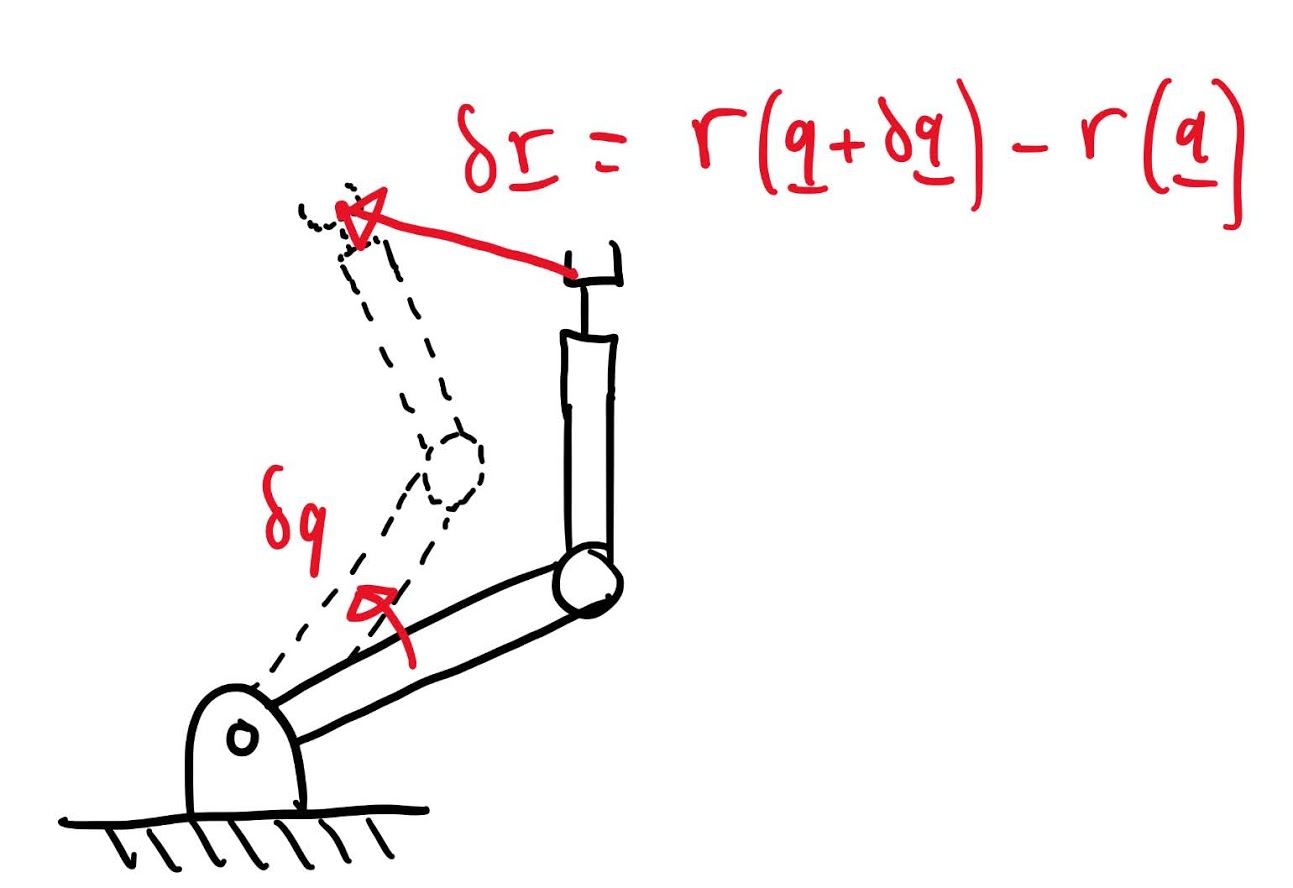
\includegraphics[width=0.5\textwidth]{diff_kin.jpg}
	\caption{Le Jacobien décrit la relation entre des déplacements infinitésimal}
	\label{fig:diff_kin_variation}
\end{figure}
%%%%%%%%%%%%%%%%%%%%%%%%%%%%%%%%%%%%%%%%%%%%%%%%%

\video{Cinématique différentielle et matrice jacobienne}{https://youtu.be/jJqYWNSsJvE}

%%%%%%%%%%%%%%%%%%%%%%%%%%%%%%%%%%%%%%%%%%%%%%%%%%%%%%%%%%%%%%%%%%%%%%%%%%%%%
\subsection{La matrice Jacobienne}
%%%%%%%%%%%%%%%%%%%%%%%%%%%%%%%%%%%%%%%%%%%%%%%%%%%%%%%%%%%%%%%%%%%%%%%%%%%%%

\paragraph{Unités} Typiquement pour les analyse de cinématique différentielle, les variables de sortie sont les DDL de translation de l'effecteur, la pose complète de l'effecteur ou bien des variables qui décrivent les DDL de l'espace de la tâche; et les variables d'entrée sont les vitesse angulaire ou linéaire des joints du robot. Les unités des composantes $J_{ij}$ de la matrice Jacobienne associée sont donc typiquement soit des unités de distance qui correspondent à des \textit{bras de levier}, ou bien des ratios adimensionnels. 

\paragraph{Non-linéarité} Il est important de noter que généralement la matrice Jacobienne est une fonction de la configuration $\col{q}$ du robot. Comme la fonction de cinématique directe est généralement hautement non-linéaire, l'effet d'un déplacement infinitésimal d'un joint sur l'effecteur dépend considérablement de la configuration initiale. La matrice Jacobienne est donc seulement valide pour décrire des petites variation déplacement autour de la configuration pour laquelle elle a été évaluée, ou bien pour la relation entre les vitesses momentanément à cette configuration. 

\paragraph{Colonnes de la matrice Jacobienne} Comme illustré à la Figure \ref{fig:jaco_graph}, dans le contexte de cinématique différentiel, la colonne $j$ de la matrice Jacobienne correspond à un vecteur déplacement infinitésimal de l'effecteur due au mouvement du joint $j$:
%%%%%%%%%%%%%%%%
\begin{equation}
J = \left[ \frac{\partial \col{r}}{\partial q_1}   \hdots \frac{\partial \col{r}}{\partial q_i} \hdots \frac{\partial \col{r}}{\partial q_n}  \right]
\end{equation}
%%%%%%%%%%%%%%%%
Chaque colonne a donc une interprétation vectorielle visuelle comme illustré à la Figure suivante.
%%%%%%%%%%%%%%%%%%%%%%%%%%%%%%%%%%%%%%%%%%%%%%%%%
\begin{figure}[H]
\vspace{-5pt}
	\centering
		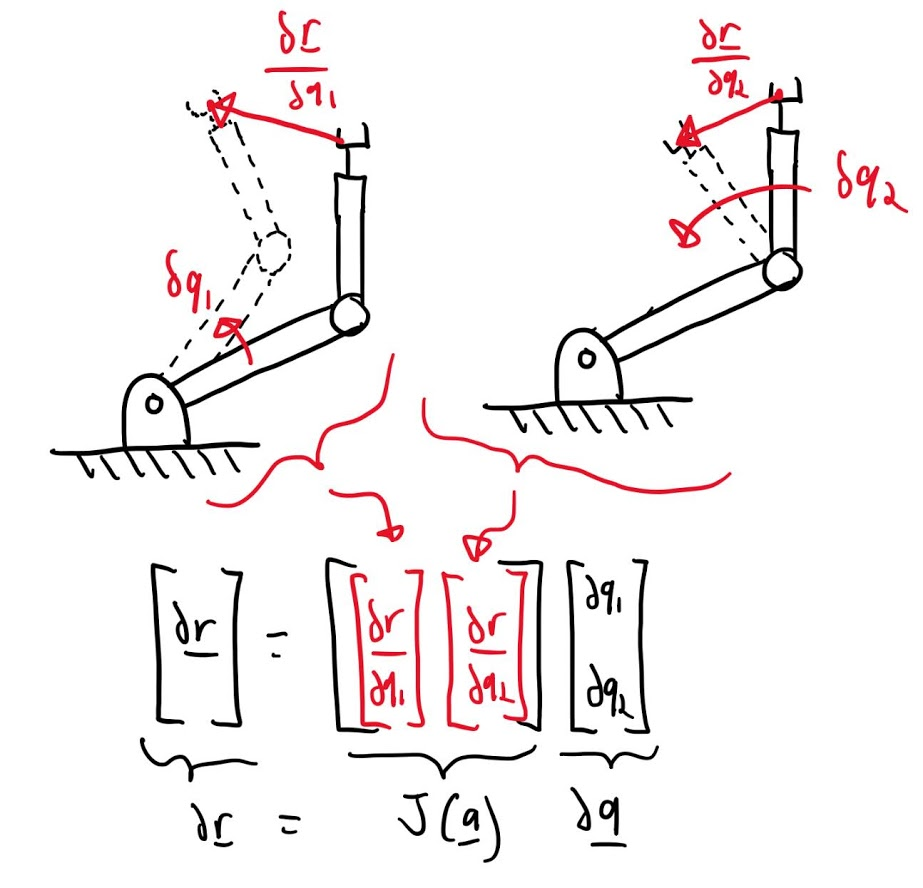
\includegraphics[width=0.65\textwidth]{jaco_graph.jpg}
	\caption{Illustration vectorielle du Jacobian du manipulateur (relation de translation)}
	\vspace{-5pt}
	\label{fig:jaco_graph}
\end{figure}
%%%%%%%%%%%%%%%%%%%%%%%%%%%%%%%%%%%%%%%%%%%%%%%%%



\paragraph{Produits vectoriels}

Lorsque l'espace de la tâche associé à un Jacobien correspond à la position cartésienne de l'effecteur d'un robot, chaque colonne du Jacobien peut aussi être déterminée basé sur un calcul vectoriel avec l'axe de rotation du joint associé. Si on considère d'abord un joint prismatique $i$, l'effet infinitésimal de son déplacement est une translation d'amplitude $\partial q_i$ dans une direction qui correspond à l'axe de translation du joint $\hat{z}_i$. Pour un joint rotatif $i$, l'effet est plutôt une rotation des membrures en aval du joint $i$ autour de l'axe de rotation du joint $\hat{z}_i$. Si on utile un repère mobile qui tourne avec toute les membrures en aval du joint $i$, les composantes de vecteurs position en aval ne varie pas, c'est la vitesse angulaire de la base vectorielle mobile qui explique la vitesse. Donc comme vue à la section \ref{sec:diffposmobilebase}, cet effet peut être représenté mathématiquement par un produit vectoriel. Le mouvement à l'effecteur (résultant de la rotation d'un axe seulement) peut donc ici être calculé par le produit vectoriel du vecteur de vitesse angulaire (l'axe de rotation fois le taux de variation de l'angle de rotation) avec le vecteur position entre l'effecteur et le centre de rotation du joint. En termes de déplacements infinitésimal de l'effecteur dus aux déplacements de joints, la relation est
%%%%%%%%%%%%%%%%
\begin{equation}
\partial \Vec{r} = \left\{ \begin{array}{c}
\left( \partial q_i \right) \, \hat{z}_i \quad \text{pour un joint $i$ prismatique}
 \\ \\
\left( \partial q_i \right) \, \hat{z}_i \, \times \, \vec{r}_{T_o/Z_i}
\quad \text{pour un joint $i$ rotatif}
\end{array}
\right.
\end{equation}
%%%%%%%%%%%%%%%%
où $q_i$ est la position du joint $i$, $\hat{z}_i$ est l'axe de rotation ou de translation du joint, $\vec{r}$ est le vecteur position de l'effecteur par rapport à une origine fixe et $\vec{r}_{T_o/Z_i}$ est le vecteur position de l'effecteur par rapport à un point d'origine $Z_i$ sur l'axe de rotation du joint $i$ (centre de rotation de ce mouvement). Cette relation vectorielle différentielle peut être utilisée pour obtenir une définition équivalente des colonnes du Jacobien: 
%%%%%%%%%%%%%%%%
\begin{equation}
\text{Colonnes du Jacobien: } \quad
\frac{\partial \col{r}}{\partial q_i} = \left\{ \begin{array}{c}
\col{z}_i \quad \text{pour un joint $i$ prismatique}
 \\ \\
\col{z}_i^{\times} \, \col{r}_{T_o/Z_i}
\quad \text{pour un joint $i$ rotatif}
\end{array}
\right.
\label{eq:jacocolprodvec}
\end{equation}
%%%%%%%%%%%%%%%%
ou toutes les composantes sont exprimée dans la base vectorielle fixe globale.


%%%%%%%%%%%%%%%%%%%%%%%%%%%%%%%%%%%%%%%%%%%%%%%%%
\begin{figure}[H]
\vspace{-5pt}
	\centering
		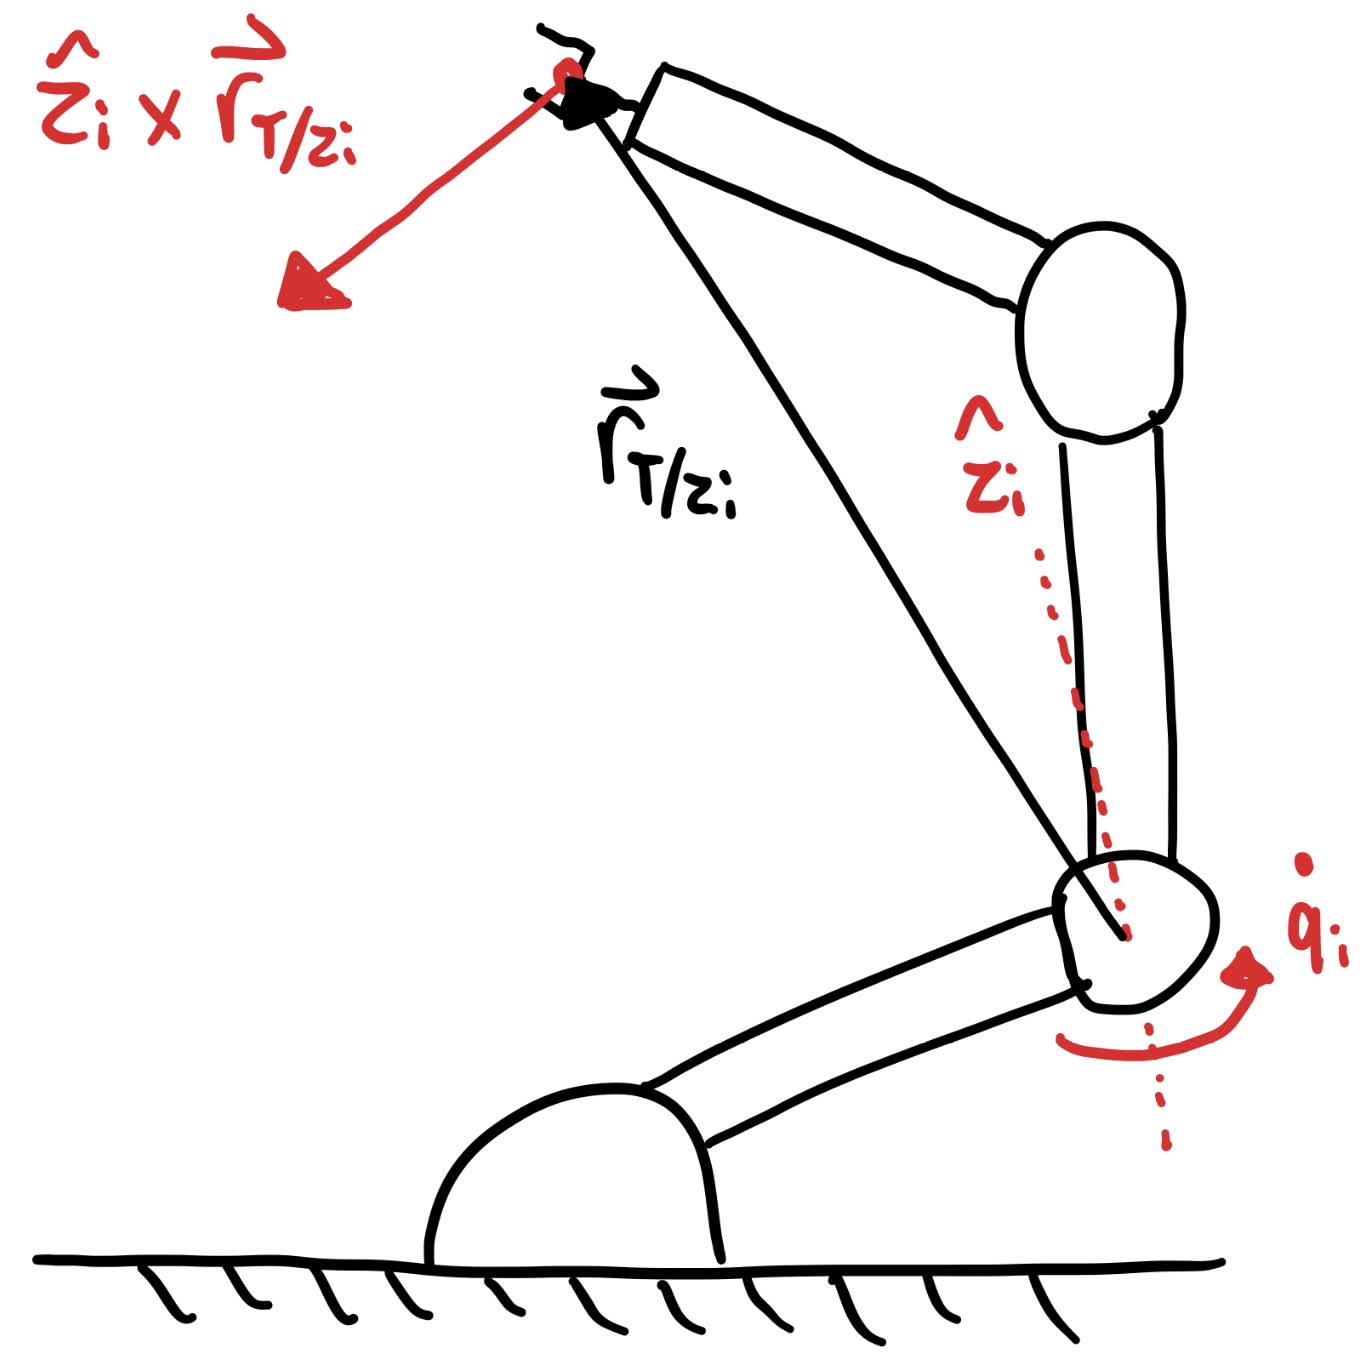
\includegraphics[width=0.40\textwidth]{jaco_vec.jpg}
	\caption{Interprétation des colonnes du Jacobian comme un poduit vectoriel}
	\vspace{-5pt}
	\label{fig:jaco_vec}
\end{figure}
%%%%%%%%%%%%%%%%%%%%%%%%%%%%%%%%%%%%%%%%%%%%%%%%%

\note{Relation avec les paramètres \textit{DH}}{
La définition des colonnes du Jacobien donnée à l'équation \eqref{eq:jacocolprodvec} est particulièrement utile pour calculer le Jacobien d'un robot manipulateur lorsqu'on a déjà déterminé les paramètres \textit{DH}. La convention de positionnement des repères fait que les axes de rotation $\col{z}_i$ et les vecteurs positions qui donnent la position des points $Z_i$ sont déjà calculés dans les matrices de transformation homogènes. Dans ce cas, cette technique peut être plus rapide que de calculer les dérivées partielles basée sur la définition donnée à l'équation \eqref{eq:matricejaco} pour construire la matrice Jacobienne.}
%En effet, le vecteur-colonne $\col{z}_i$ correspond à la troisième colonne de la matrice de rotation $^{w}R^z$ qui donne l'orientation du lien rigide en aval du joint $i$ par rapport à la base vectorielle globale fixe. 



\paragraph{Cinématique différentielle pour l'orientation de l'effecteur}

Lorsque ce n'est pas la position cartésienne de l'effecteur que l'on désire contrôler mais plutôt sont orientation, le vecteur sortie $\col{\dot{r}}$ contient alors les composantes du vecteur de vitesse angulaire de l'effecteur qui définie le taux de variation de l'orientation d'une base vectorielle $t$ fixée sur l'effecteur par rapport à une base fixe $a$ par rapport à la base du robot manipulateur. L'équation de cinématique différentiel est alors caractérisé par l'addition des vecteurs de vitesse angulaire relative pour chacun des joints d'un système, basée sur l'équation \eqref{eq:angspeedadd}, pour un robot à 6 joints:
%%%%%%%%%%%%%%%%
\begin{align}
\vec{w}_{t/w} = \vec{w}_{t/f} + \vec{w}_{f/e} + \vec{w}_{e/d} + \vec{w}_{d/c} + \vec{w}_{c/b} + \vec{w}_{b/a} 
\end{align}
%%%%%%%%%%%%%%%%
où les base $b$, $c$, $d$, $e$ et $f$ sont des bases vectorielles intermédiaires sur les joints (voire Figure \ref{fig:serial_kin_3}).
Donc le cas commun où le robot manipulateur a seulement des joints rotatifs à un degrée de liberté, chacun vecteur de vitesse angulaire est simplement l'axe de rotation $\hat{z}_i$ fois de taux de variation de l'angle: 
%%%%%%%%%%%%%%%%
\begin{align}
\vec{w}_{t/w} &= \hat{z}_6 \dot{q}_6 +  \hat{z}_5 \dot{q}_5 +  \hat{z}_4 \dot{q}_4 +  \hat{z}_3 \dot{q}_3 +  \hat{z}_2 \dot{q}_2 +  \hat{z}_1 \dot{q}_1 \\
\col{w} &= 
\underbrace{
\left[ \, \col{z}_1 \, \col{z}_2 \, \col{z}_3 \, \col{z}_4 \, \col{z}_5 \, \col{z}_6 \, \right]  
}_{J_{ori}}
\, \col{\dot{q}} 
\end{align}
%%%%%%%%%%%%%%%%
Dans ce cas, les colonnes du Jacobien sont simplement les axes de rotation de chacun des joints. Pour des joints prismatiques, ils n'influencent pas l'orientation de l'effecteur et les colonnes du Jacobien associées à un joint prismatique sont donc nulles:
%%%%%%%%%%%%%%%%
\begin{equation}
\text{Colonnes du Jacobien (orientation): } \quad\left\{ \begin{array}{c}
\col{0} \quad \text{pour un joint $i$ prismatique}
 \\ \\
\col{z}_i \quad \text{pour un joint $i$ rotatif}
\end{array}
\right.
\end{equation}
%%%%%%%%%%%%%%%%
%
Un exemple où on s'intéresserait plutôt à l'orientation de système robotique, serait pour asservir une antenne de communication qui doit toujours être alignée avec un satellite. Dans ce cas, l'effecteur du système est la parabole de l'antenne et c'est sont orientation spatiale qui est importante seulement. 

\paragraph{Cinématique différentielle pour la pose de l'effecteur}

Si on désire décrire de taux de variation de la pose complète de l'effecteur, il suffit de combiner les systèmes linéaire la translation et l'orientation:
%%%%%%%%%%%%%%%%
\begin{align}
\col{\dot{r}} &= \left[ J_{trans} \right]  \, \col{\dot{q}} \quad \quad 
J_{trans} = \left[ \hdots \col{z}_i^{\times} \, \col{r}_{T_o/Z_i}  \hdots  \right] \\
\col{w} &= \left[ J_{ori} \right]  \, \col{\dot{q}} \quad \quad 
J_{ori}   = \left[ \hdots   \col{z}_i  \hdots  \right] \\
\left[  \begin{array}{c}
\col{\dot{r}} \\ \col{w}
\end{array} \right] &= \left[ J_{pose} \right]  \, \col{\dot{q}} \quad \quad 
J_{pose}  = \left[ \begin{array}{c}
J_{trans} \\ J_{ori} 
\end{array} \right] 
\end{align}
%%%%%%%%%%%%%%%%


\paragraph{Cinématique différentielle pour un espace de la tâche}

Il est aussi possible de définir un matrice Jacobienne pour une relation spécifique à une tâche. Par exemple, voir Figure \ref{fig:spaces}, où il serait désirable d'obtenir les équations qui relit la position/vitesse des joints et celle de la tâche décrite en termes de $x$ et $y$ sur un plan particulier. Si on a un espace de la tâche de dimension $m$ (normalement égale ou inférieur au nombre de DDL de l'effecteur du robot), alors on peut déterminer matrice Jacobienne $m$ par $n$. 
%%%%%%%%%%%%%%%%
\begin{align}
\Big[ \col{r}_{e} \Big]_{m \times 1} = f_{e}( \col{q} )
\quad \Rightarrow \quad 
\Big[ \col{\dot{r}_{e}}\Big]_{m \times 1} &= \Big[ J_{e} \Big]_{m \times n}  \, \Big[ \col{\dot{q}} \Big]_{n \times 1}
\end{align}
%%%%%%%%%%%%%%%%

\note{Note de lecture}{
Pour les sections suivantes, s'il n'est pas préciser autrement on va toujours travailler avec la relation cinématique de translation seulement de l'effecteur pour l'explication des concepts. Les exemples sont visuellement plus clair dans cette situation. Toutefois, tout les concepts présentés se généralisent à toutes les situations.
}

\newpage
%%%%%%%%%%%%%%%%%%%%%%%%%%%%%%%%%%%%%%%%%%%%%%%%%%%%%%%%%%%%%%%%%%%%%%%%%%%%%%%%%%%%%%%%%%%%%%%%%
%\subsection{Exemples de cinématique différentielle pour des robots manipulateurs}

\video{Exemple de calcul de la matrice jacobienne}{https://youtu.be/qgqDscXSsMM}

%%%%%%%%%%%%%%%%%%%%%%%%%%%%%%%%%%%%%%%%%%%%%%%%%%%%%%%%%%%%%%%%%%%%%%%%%%%%%%%%%%%%%%%%%%%%%%%%%
\begin{example}[Cinématique différentielle d'un robot cartésien]

La Figure \ref{fig:jaco_robot_cart} illustre un robot planaire constitué de deux actionneurs linéaires basé sur des vis à billes qui sont assemblés à 90 degrées. 
%%%%%%%%%%%%%%%%%%%%%%%%%%%%%%%%%%%%%%%%%%%%%%%%%
\begin{figure}[H]
	\vspace{-5pt}
	\centering
		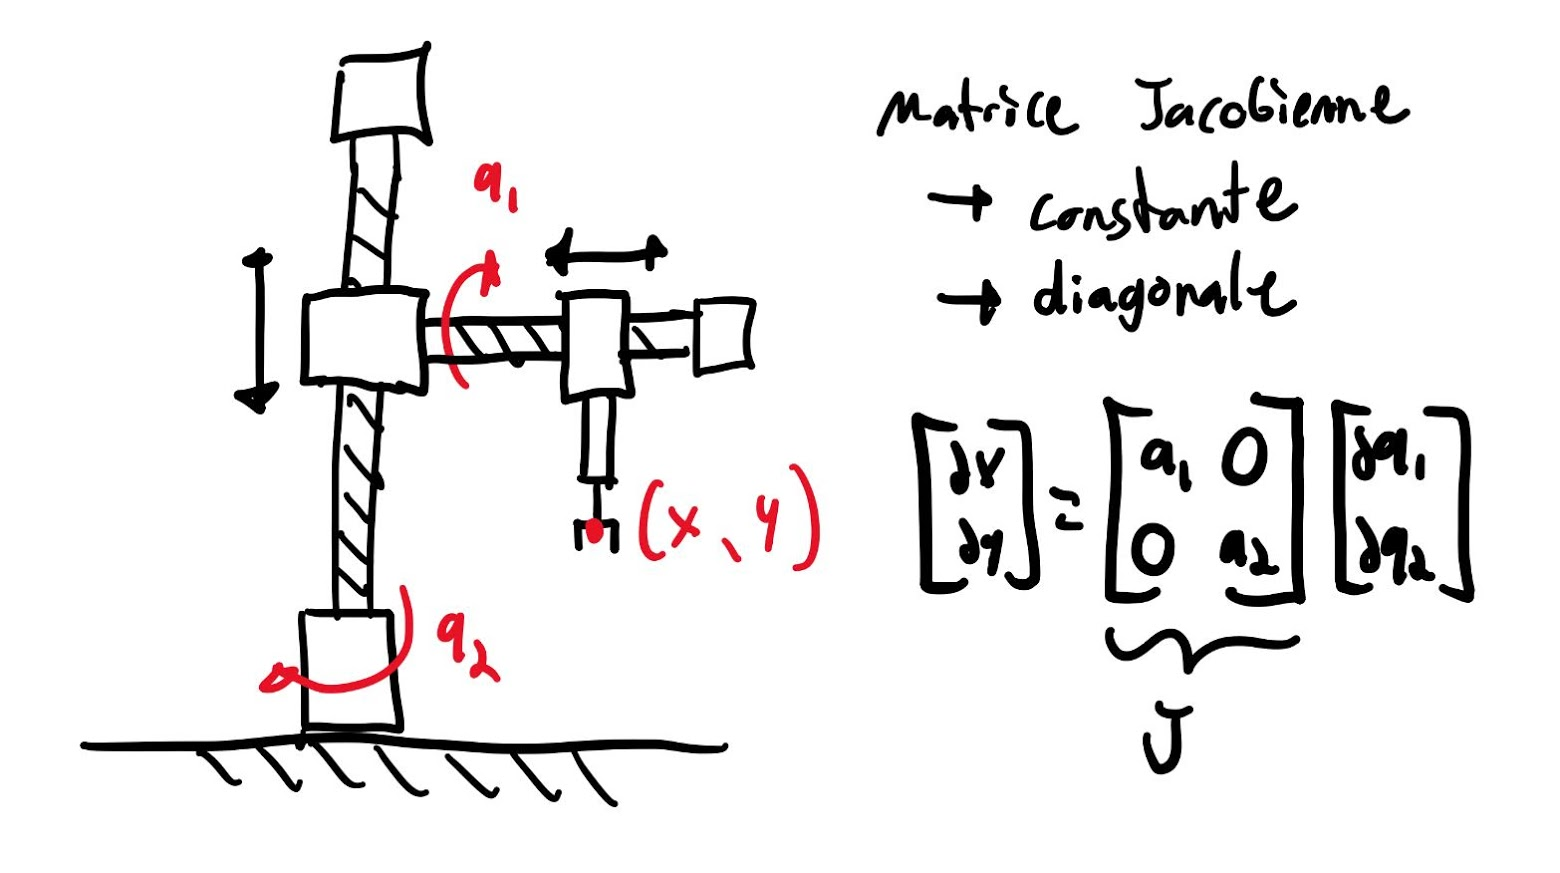
\includegraphics[width=0.65\textwidth]{jaco_robot_cart.jpg}
	\caption{Jacobien pour un robot cartésien}
	\vspace{-5pt}
	\label{fig:jaco_robot_cart}
\end{figure}
%%%%%%%%%%%%%%%%%%%%%%%%%%%%%%%%%%%%%%%%%%%%%%%%%

Pour ce robot, chaque actionneur linéaire contrôle de façon indépendante la translation $x$ et $y$ de l'effecteur, la fonction de cinématique directe est donnée par :
%%%%%%%%%%%%%%%%
\begin{align}
\quad \col{r} &= f\left( \, \col{q} \, \right)  \\
\left[ \begin{array}{c} x \\ y  \end{array} \right]  &= \left[ \begin{array}{c} a_1 q_1 \\ a_2 q_2  \end{array} \right]
\label{eq:fwdkinlin}
\end{align}
%%%%%%%%%%%%%%%
ou les variables $a_i$ sont des constantes qui relient la rotation angulaire des vis aux déplacements linéaires. La relation différentielle peut alors être calculée:
%%%%%%%%%%%%%%%%%%%%%%%%%%%%%%%%%%%
\begin{align}
\underbrace{ \left[ \begin{array}{c} \dot{x} \\ \dot{y}  \end{array} \right] }_{\dot{\col{r}}}
 &= 
\underbrace{ \left[ \begin{array}{c c } 
\frac{\partial x }{\partial q_1}   & \frac{\partial x }{\partial q_2} \\ 
\frac{\partial y }{\partial q_1}   & \frac{\partial y }{\partial q_2}
\end{array} \right]  }_{ J } 
\underbrace{ \left[ \begin{array}{c} 
\dot{q}_1 \\ 
\dot{q}_2 
\end{array} \right]}_{ \dot{\col{q}} } \\
%%%%%%%%%%%%%
\underbrace{ \left[ \begin{array}{c} \dot{x} \\ \dot{y}  \end{array} \right] }_{\dot{\col{r}}}
 &= 
\underbrace{ \left[ \begin{array}{c c } 
a_1 & 0 \\ 
0   & a_2
\end{array} \right]  }_{ J } 
\underbrace{ \left[ \begin{array}{c} 
\dot{q}_1 \\ 
\dot{q}_2 
\end{array} \right]}_{ \dot{\col{q}} } \\
\end{align} 
%%%%%%%%%%%%%%%%%%%%%%%%%%%%%%%%%%%

Il est a noter ici que: \textbf{1)} la matrice Jacobienne est diagonale car chaque joint influence indépendamment un seul DDL de l'effecteur. \textbf{2)} la matrice Jacobienne est constante et indépendante de $\col{q}$ car la relation de cinématique directe, voir équation \eqref{eq:fwdkinlin}, est linéaire. 
%%%%%%%%%%%%%%%%%%%%%%%%%%%%%%%%%%%
\end{example}

%%%%%%%%%%%%%%%%%%%%%%%%%%%%%%%%%%%%%%%%%%%%%%%%%%%%%%%%%%%%%%%%%%%%%%%%%%%%%%%%%%%%%%%%%%%%%%%%%%%%%%%%%
\begin{example}[Cinématique différentielle d'un robot à deux joints]

\label{sec:kindiff_2dof}

%%%%%%%%%%%%%%%%%%%%%%%%%%%%%%%%%%%%%%%%%%%%%%%%%
\begin{figure}[H]
	\centering
		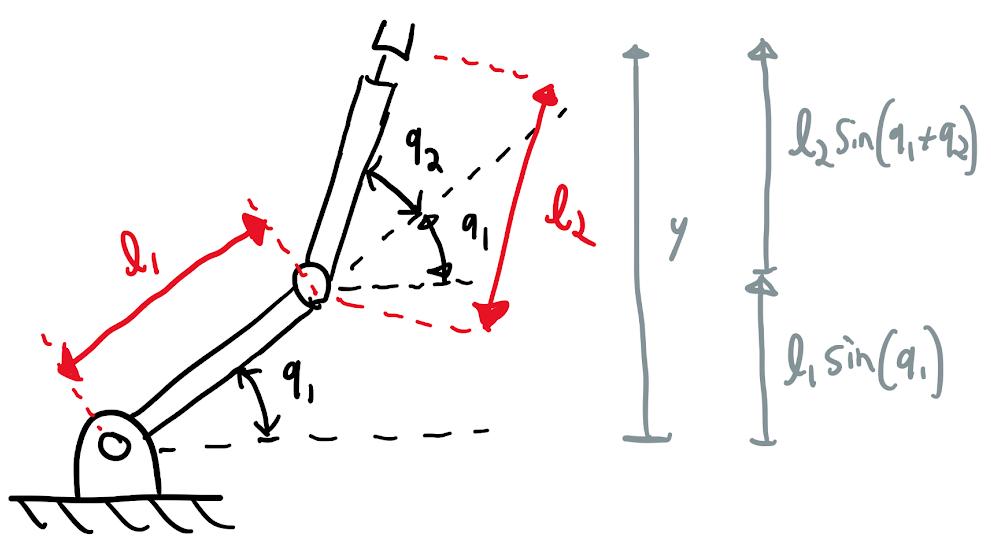
\includegraphics[width=0.65\textwidth]{robot_2dof.png}
	\caption{Robot à deux joints}
	\label{fig:robot_2dof}
\end{figure}
%%%%%%%%%%%%%%%%%%%%%%%%%%%%%%%%%%%%%%%%%%%%%%%%%

Pour un robot manipulateur planaire à deux DDL, comme illustré à la Figure \ref{fig:robot_2dof}, la fonction de cinématique directe est données par:
%%%%%%%%%%%%%%%%%%%%%%%%%%%%%%%%%%%
\begin{align}
\col{r} &= \left[ \begin{array}{c} x \\ y  \end{array} \right]  = \left[ \begin{array}{c} 
 l_1 c_1 + l_2 c_{12} \\ 
 l_1 s_1 + l_2 s_{12}  
\end{array} \right] 
\label{eq:kinfwd2dof}
\end{align} 
%%%%%%%%%%%%%%%%%%%%%%%%%%%%%%%%%%%
avec
%%%%%%%%%%%%%%%%%%%%%%%%%%%%%%%%%%%
\begin{align}
c_1    &= \cos( q_1 ) \\
s_1    &= \sin( q_1 ) \\
c_{12} &= \cos( q_1 + q_2 ) \\
s_{12} &= \sin( q_1 + q_2 )
\end{align} 
%%%%%%%%%%%%%%%%%%%%%%%%%%%%%%%%%%%

On peut alors trouver la relation différentielle en dérivant par rapport au temps:
%%%%%%%%%%%%%%%%%%%%%%%%%%%%%%%%%%%
\begin{align}
\dot{\col{r}} &= \frac{d\col{r}}{dt} = \left[ \begin{array}{c} \dot{x} \\ \dot{y}  \end{array} \right]  = \left[ \begin{array}{c} 
-l_1 s_1 \dot{q}_1 - l_2 s_{12}( \dot{q}_1 + \dot{q}_2 ) \\ 
 l_1 c_1 \dot{q}_1 + l_2 c_{12}( \dot{q}_1 + \dot{q}_2 )  
\end{array} \right] \\
\dot{\col{r}}  &= 
\underbrace{ \left[ \begin{array}{c c } 
-l_1 s_1 - l_2 s_{12} & - l_2 s_{12} \\ 
 l_1 c_1 + l_2 c_{12} &   l_2 c_{12}
\end{array} \right]  }_{ J(\col{q}) } 
\underbrace{ \left[ \begin{array}{c} 
\dot{q}_1 \\ 
\dot{q}_2 
\end{array} \right]}_{ \dot{\col{q}} } \\
\dot{\col{r}}  &= J(\col{q}) \dot{\col{q}}
\end{align} 
%%%%%%%%%%%%%%%%%%%%%%%%%%%%%%%%%%%
\end{example}



%%%%%%%%%%%%%%%%%%%%%%%%%%%%%%%%%%%%%%%%%%%%%%%%%%%%%%%%%%%%%%%%%%%%%%%%%%%%%%%%%%%%%%%%%%%%%%%%%%%%%%%%%
\begin{example}[Cinématique différentielle d'un robot à trois joints]
\label{sec:diffkinrobot3dofex}

Les Figures \pageref{fig:jaco_3dof_a} et \ref{fig:jaco_3dof_b} illustre la cinématique différentielle d'un robot à trois joints dans une configuration qui permet de bien visualiser indépendamment les effets du mouvement de chaque joint. 

%%%%%%%%%%%%%%%%%%%%%%%%%%%%%%%%%%%%%%%%%%%%%%%%%
\begin{figure}[H]
	\centering
		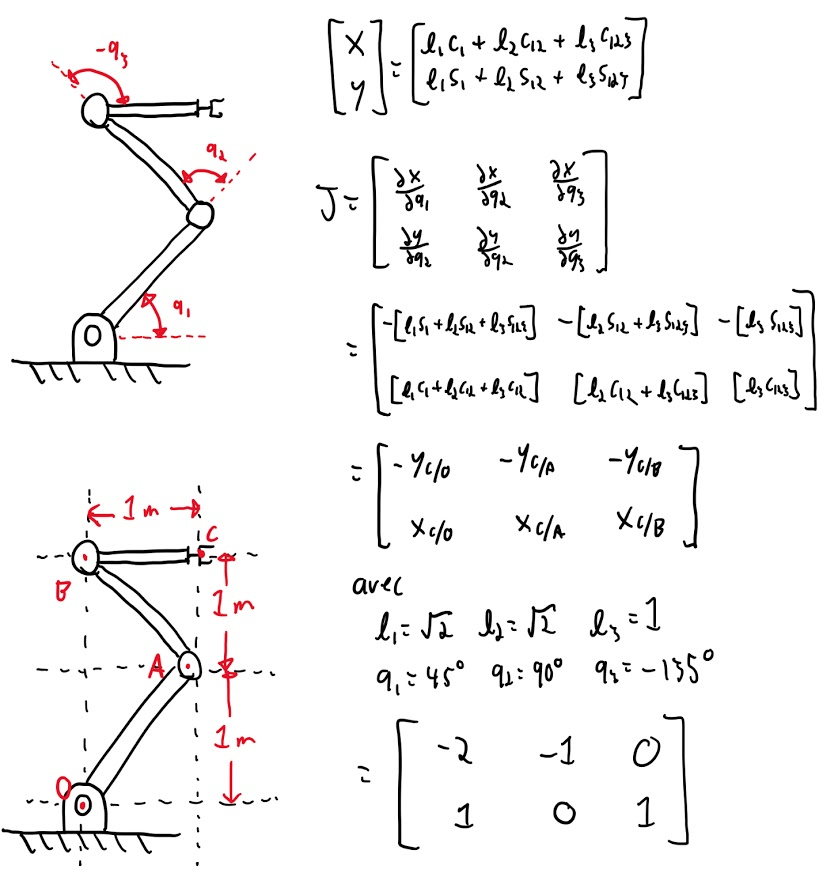
\includegraphics[width=0.75\textwidth]{jaco_3dof_a.jpg}
	\caption{Jacobien d'un robot à trois joints - partie a)}
	\label{fig:jaco_3dof_a}
\end{figure}
%%%%%%%%%%%%%%%%%%%%%%%%%%%%%%%%%%%%%%%%%%%%%%%%%

%%%%%%%%%%%%%%%%%%%%%%%%%%%%%%%%%%%%%%%%%%%%%%%%%
\begin{figure}[H]
	\centering
		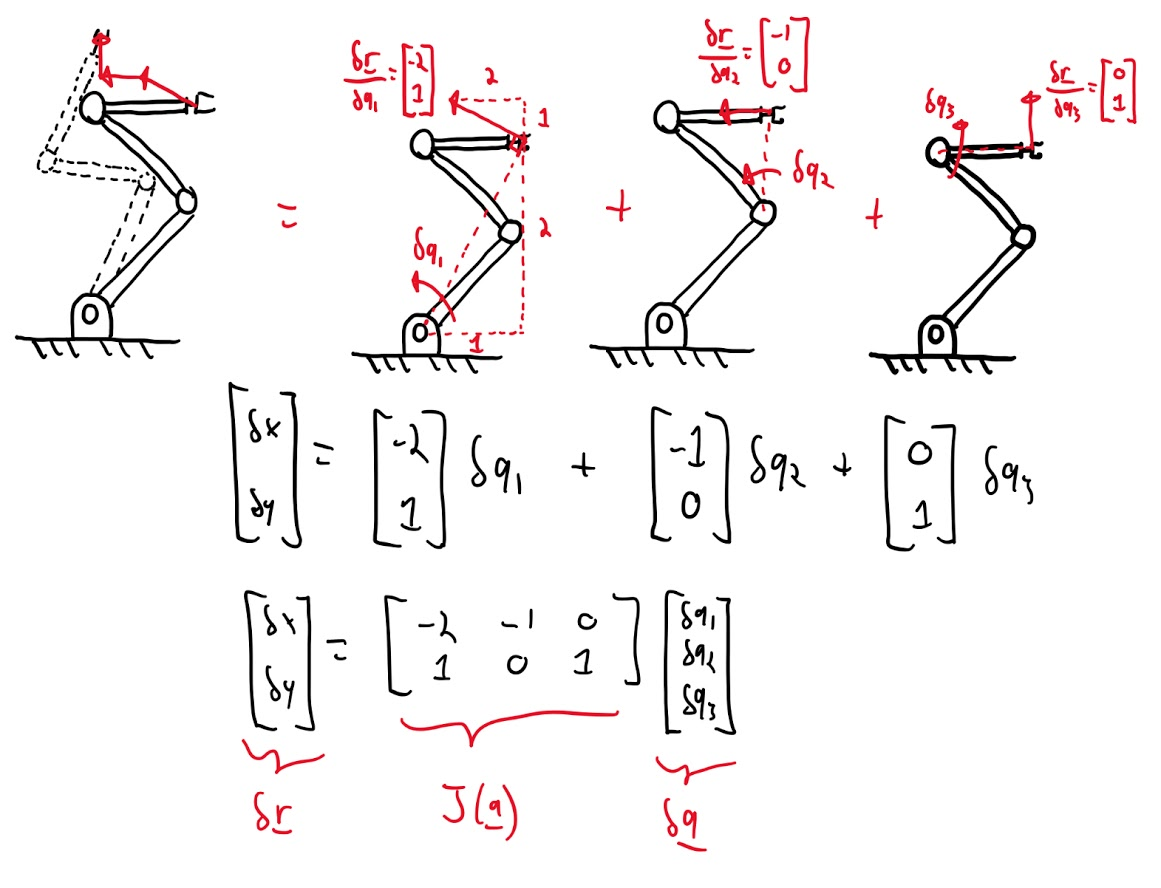
\includegraphics[width=0.85\textwidth]{jaco_3dof_b.jpg}
	\caption{Jacobien d'un robot à trois joints - partie b)}
	\label{fig:jaco_3dof_b}
\end{figure}
%%%%%%%%%%%%%%%%%%%%%%%%%%%%%%%%%%%%%%%%%%%%%%%%%
\end{example}


%%%%%%%%%%%%%%%%%%%%%%%%%%%%%%%%%%%%%%%%%%%%%%%%%%%%%%%%%%%%%%%%%%%%%%%%%%%%%%%%%%%%%%%%%%%%%%%%%%%%%%%%%
\newpage
\section{Cinématique différentielle inverse}

Lorsque le problème de cinématique différentielle est inversé, c'est-à-dire lorsqu'on cherche un vecteur de vitesse aux joints $\col{\dot{q}}$ qui va produire une vitesse de l'effecteur spécifiée $\col{\dot{r}}$, il faut inverser la relation mathématique. Lorsque la matrice Jacobienne est carré et non-singulière, il suffit de multiplier la relation $\col{\dot{r}} = J\left( \, \col{q} \, \right) \, \col{\dot{q}}$ par l'inverse du Jacobien des deux côtés de l'équation pour obtenir la relation:
%
%%%%%%%%%%%%%%%%%%%%%%%%%%%%%%%%%%%
\begin{align}
\col{\dot{q}} = J^{-1}\left( \, \col{q} \, \right) \, \col{\dot{r}}
\end{align} 
%%%%%%%%%%%%%%%%%%%%%%%%%%%%%%%%%%%
%
Toutefois, cette opération est impossible si le robot a une configuration singulière (voir section \ref{sec:singu}). De plus, si les dimensions de $\col{q}$ et $\col{r}$ sont différentes, la matrice Jacobienne est rectangulaire et d'autres techniques doivent être utilisée (voir sections \ref{sec:invdiffkinredondant} et \ref{sec:overconstraintrobot})

\video{Cinématique différentielle inverse des robots manipulateurs}{https://youtu.be/YqYV10mVVBI}


%%%%%%%%%%%%%%%%%%%%%%%%%%%%%%%%%%%%%%%%%%%%%%%%%%%%%%%%%%%%%%%%%%%%%%%%%%%%%%%%%%%%%%%%%%%%%%%%%%%%%%%%%
\subsection{Les singularités}
\label{sec:singu}
%%%%%%%%%%%%%%%%%%%%%%%%%%%%%%%%%%
Certaine configuration $\col{q}$ d'un robot manipulateur peuvent être singulière, c'est-à-dire des configuration pour lesquelles il est impossible d'inverser la matrice Jacobienne. Les configurations singulière sont l'ensemble des configurations pour lesquelles le déterminant de la matrice Jacobienne est nul:
%%%%%%%%%%%%%%%%%%%%%%%%%%%%%%%%%%%
\begin{align}
\text{Singularités :} \quad \{  \col{q} \; | \; det(J(\col{q})) = 0 \}
\end{align} 
%%%%%%%%%%%%%%%%%%%%%%%%%%%%%%%%%%%
Ces situations correspondent aussi à lorsque les colonnes de $J$ sont co-linéaires, et qu'aucune combinaison linéaire ne permet de déplacer l'effecteur dans au moins une direction (la matrice jacobienne a un espace-nul gauche, voir section \ref{sec:leftnullspace} pour les notions d'algèbre linéaire associées). 


\begin{example}[Singularités d'un robot manipulateur planaire à 2 joints]

Pour un robot manipulateur à deux DDl comme décrit à l'exemple \ref{sec:kindiff_2dof}, le Jacobien est donné par:
%%%%%%%%%%%%%%%%%%%%%%%%%%%%%%%%%%%
\begin{align}
J = \left[ \begin{array}{c c} 
-(l_1 s_1 + l_2 s_{12}) & - l_2 s_{12} \\
 (l_1 c_1 + l_2 c_{12}) &   l_2 c_{12}
\end{array} \right]
\end{align} 
%%%%%%%%%%%%%%%%%%%%%%%%%%%%%%%%%%%
Le déterminant de la matrice est donnée par:
%%%%%%%%%%%%%%%%%%%%%%%%%%%%%%%%%%%
\begin{align}
det(J) &= l_2 s_{12} (l_1 c_1 + l_2 c_{12}) - l_2 c_{12} (l_1 s_1 + l_2 s_{12}) \\
       &= l_1 l_2 s_{12} c_1 + l_2^2 s_{12} c_{12} - l_1 l_2 s_1 c_{12} - l_2^2 s_{12} c_{12} \\
			 &= l_1 l_2 ( s_1 c_{12} - c_1 s_{12} ) \\
			 &= l_1 l_2 s_2
\end{align} 
%%%%%%%%%%%%%%%%%%%%%%%%%%%%%%%%%%%

Donc les singularités sont les configurations avec un angle $q_2$ égale à 0 ou 180 degrés. Comme illustré à la Figure \ref{fig:sigularite_2dof}, ces configurations correspondent à lorsque les deux liens rigides du robot sont alignés. Dans ces configurations, il est seulement possible de faire bouger l'effecteur dans une direction perpendiculaire aux liens rigides. Comme illustré à la Figure \ref{fig:sigularite_2dof_b}, la direction pour laquelle le mouvement est possible correspond à l'espace colonne de la matrice Jacobienne, et la direction orthogonale pour laquelle il est impossible de déplacer l'effecteur correspond au left-nullspace de la matrice Jacobienne, voir section \ref{sec:4espfond} pour les notions d'algèbre linéaire associées.

%%%%%%%%%%%%%%%%%%%%%%%%%%%%%%%%%%
\begin{figure}[H]
	\centering
		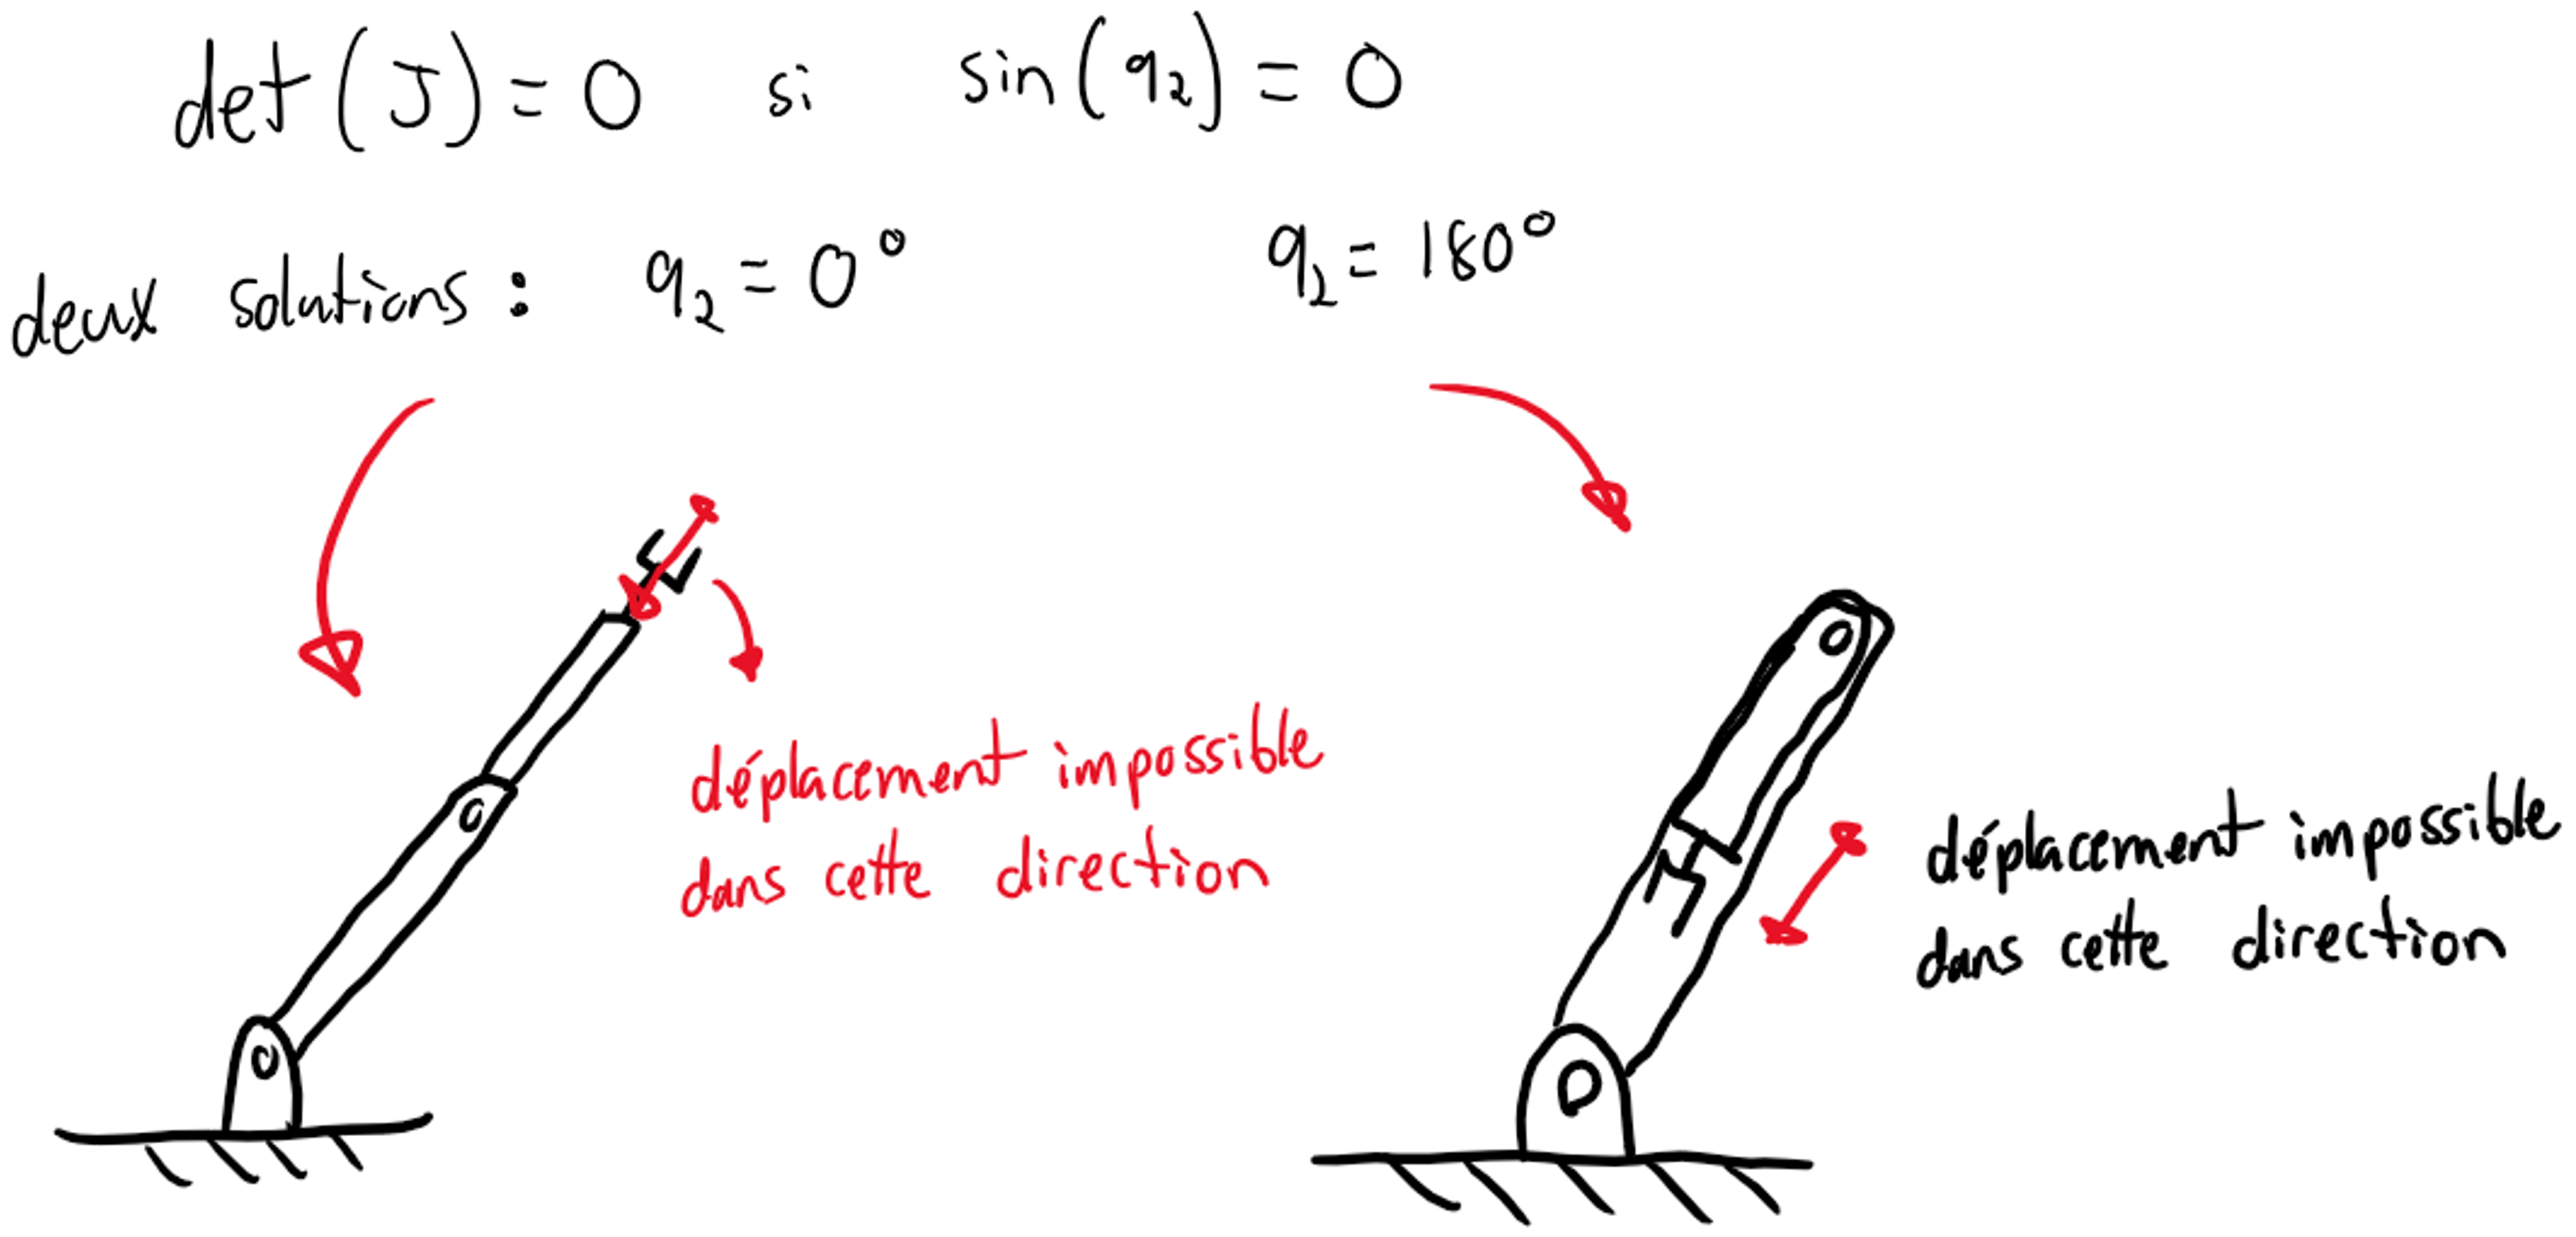
\includegraphics[width=0.75\textwidth]{sigularite_2dof.png}
	\caption{Singularités pour un robot manipulateur à deux DDL}
	\label{fig:sigularite_2dof}
\end{figure}
%%%%%%%%%%%%%%%%%%%%%%%%%%%%%%%%%%

%%%%%%%%%%%%%%%%%%%%%%%%%%%%%%%%%%
\begin{figure}[H]
	\centering
		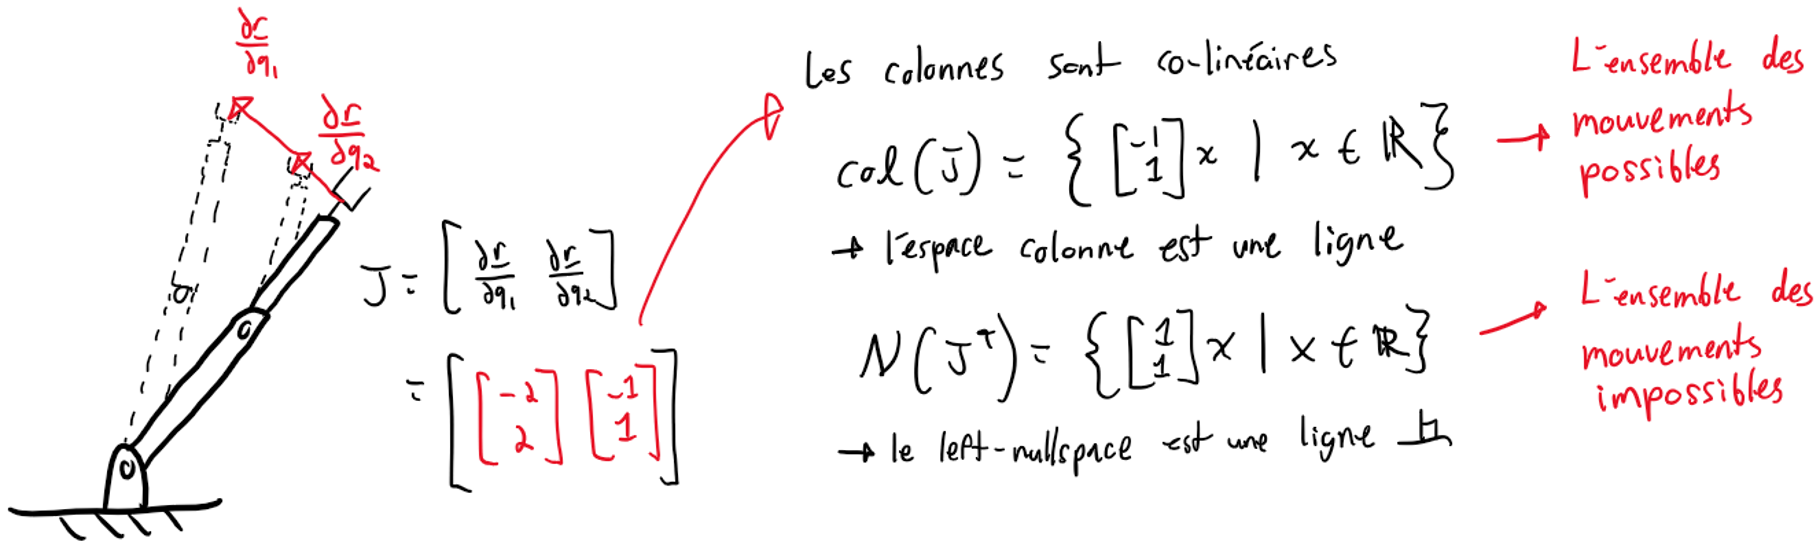
\includegraphics[width=0.95\textwidth]{sigularite_2dof_b.png}
	\caption{Co-linéarité des colonnes du Jacobien pour une singularité}
	\label{fig:sigularite_2dof_b}
\end{figure}
%%%%%%%%%%%%%%%%%%%%%%%%%%%%%%%%%%

\end{example}

\subsubsection{Limites de l'espace de travail}

Un robot va nécessairement être sur une singularité aux limites de sont espace de travail, car par définition le robot est incapable de bouger son effecteur dans la direction normale à la surface qui définie la limite de l'espace de travail (sinon le robot pourrait sortir de l'espace de travail ce qui est une contradiction). Par exemple, les deux singularité du robot 2DDL de l'exemple précédant correspondent à des configurations où l'effecteur est à la limite intérieur de l'espace de travail ou à la limite extérieur de l'espace de travail. 


\subsubsection{Types de singularités}

Détails à venir!


%%%%%%%%%%%%%%%%%%%%%%%%%%%%%%%%%%%%%%%%%%%%%%%%%%%%%%%%%%%%%%%%%%%%%%%%%%%%%%%%%%%%%%%%%%%%%%%%%%%%%%%%%
\subsection{Cinématique différentielle inverse d'un robot redondant (situations sous-contraintes)}
\label{sec:invdiffkinredondant}
%%%%%%%%%%%%%%%%%%%%%%%%%%%%%%%%%%

Si le nombre d'entrées $n$ est plus grand que le nombre de sorties $m$ : 
%%%%%%%%%%%%%%%%%%%%%%%%%%%%%%%%%%%
\begin{align}
n > m
\end{align} 
%%%%%%%%%%%%%%%%%%%%%%%%%%%%%%%%%%%
avec 
%%%%%%%%%%%%%%%%%%%%%%%%%%%%%%%%%%%
\begin{align}
n &= dim(\col{q}) = \quad\text{Nombre de DDL du robot} \\
m &= dim(\col{r}) = \quad\text{Coordonnées de l'espace de la tâche} 
\end{align} 
%%%%%%%%%%%%%%%%%%%%%%%%%%%%%%%%%%%
le robot est dit redondant, et le problème de cinématique différentiel inverse est sous-contraint: il y a plusieurs solutions possible de déplacement des joints qui produisent un même déplacement de l'effecteur. Le Jacobien d'une telle situation est rectangulaire, il a plus de colonnes que de rangées:
%%%%%%%%%%%%%%%%%%%%%%%%%%%%%%%%%%%
\begin{align}
\left[ \begin{array}{c}  \\ \dot{\col{r}} \\ \\
\end{array} \right]_{m \times 1}
&= 
\left[ \begin{array}{c c c c c} 
&&&&\\
&& J(\col{q}) &&\\
&&&&
\end{array} \right]_{m \times n}
\left[ \begin{array}{c} 
\\ \\ \dot{\col{q}} \\ \\ \\
\end{array} \right]_{n \times 1}
\label{eq:underconstraintdiffkin}
\end{align} 
%%%%%%%%%%%%%%%%%%%%%%%%%%%%%%%%%%%
Cette situation nous même à un problème d'algèbre linéaire sous-contraint qui peu être résolu avec une méthode qui utilise une matrice pseudo inverse, voir section \ref{sec:pseudoinverse} pour les notions d'algèbre linéaire. Cette situation est aussi caractérisée par la présence d'un nullspace: une combinaison de déplacement des joints peut avoir un effet net nul sur l'effecteur, voir section \ref{sec:nullspace} pour les notions d'algèbre linéaire et l'exemple \ref{fig:4spaces_ex1}. 

Une méthode pour travailler avec ce genre de situation consiste à utiliser l'équation de cinématique inverse suivante:
%%%%%%%%%%%%%%%%%%%%%%%%%%%%%%%%%%%
\begin{align}
\left[ \begin{array}{c}  \\ \\ \dot{\col{q}} \\ \\ \\
\end{array} \right]_{n \times 1}
&= 
\underbrace{
\left[ \begin{array}{c c c} 
&&\\ &&\\ & J^{\#} & \\&& \\ &&
\end{array} \right]_{n \times m}
}_{\text{Pseudo-inverse}}
\left[ \begin{array}{c} 
\\ \dot{\col{r}} \\ \\
\end{array} \right]_{m \times 1} + 
\underbrace{
\left[ \begin{array}{c c c c c} 
&&&&\\ &&&&\\ && I - J^{\#}J && \\&&&& \\ &&&&
\end{array} \right]_{n \times n}
}_{\text{Projection sur le Nullspace}}
\left[ \begin{array}{c} 
\\ \\ \col{\psi} \\ \\ \\
\end{array} \right]_{n \times 1}
\label{eq:pseudoinversediffkin}
\end{align} 
%%%%%%%%%%%%%%%%%%%%%%%%%%%%%%%%%%%
avec $J^{\#}$ qui est la matrice pseudo-inverse droite de Moore–Penrose, définie par:
%%%%%%%%%%%%%%%%%%%%%%%%%%%%%%%%%%%
\begin{align}
J^{\#} = J^T\, (JJ^T)^{-1}
\end{align} 
%%%%%%%%%%%%%%%%%%%%%%%%%%%%%%%%%%%
Le premier terme $J^{\#} \col{\dot{r}}$ produit un vecteur $\col{\dot{q}}$ qui produit une solution exacte pour le système d'équations \eqref{eq:underconstraintdiffkin}
et minimise la norme du vecteur-colonne $\col{\dot{q}}$. Le second terme produit une variation pour le vecteur $\col{\dot{q}}$ qui réside dans l'espace nul de la matrice $J$, donc cette variation n'a aucun influence sur la sortie et n’affectera pas l'objectif principal d'obtenir un vecteur $\col{\dot{q}}$ qui produit un mouvement de l'effecteur donné par $\col{\dot{r}}$. Le vecteur $\col{\psi}$ dans le second terme est arbitraire et peut être utilisé pour prioriser certaine solutions sans influencer la justesse de la solution. 


%%%%%%%%%%%%%%%%%%%%%%%%%%%%%%%%%%%%%%%%%%%%%%%%%%%%%%%%%%%%%%%%%%%%%%%%%%%%%%%%%%%%%%%%%%%%%%%%%%%%%%%%%
\begin{example}[Exemple de cinématique différentielle inverse pour une situation sous-contrainte]
Le robot de l'exemple \ref{sec:diffkinrobot3dofex} est ici analysé en termes de cinématique différentielle, la Figure \ref{fig:robot_redo_a} illustre la présence de plusieurs solutions possibles et la Figure \ref{fig:robot_redo_c} illustre l'utilisation de la matrice pseudo-inverse pour obtenir la solution optimale ainsi que le nullspace. 
%
%%%%%%%%%%%%%%%%%%%%%%%%%%%%%%%%%%
\begin{figure}[H]
	\centering
		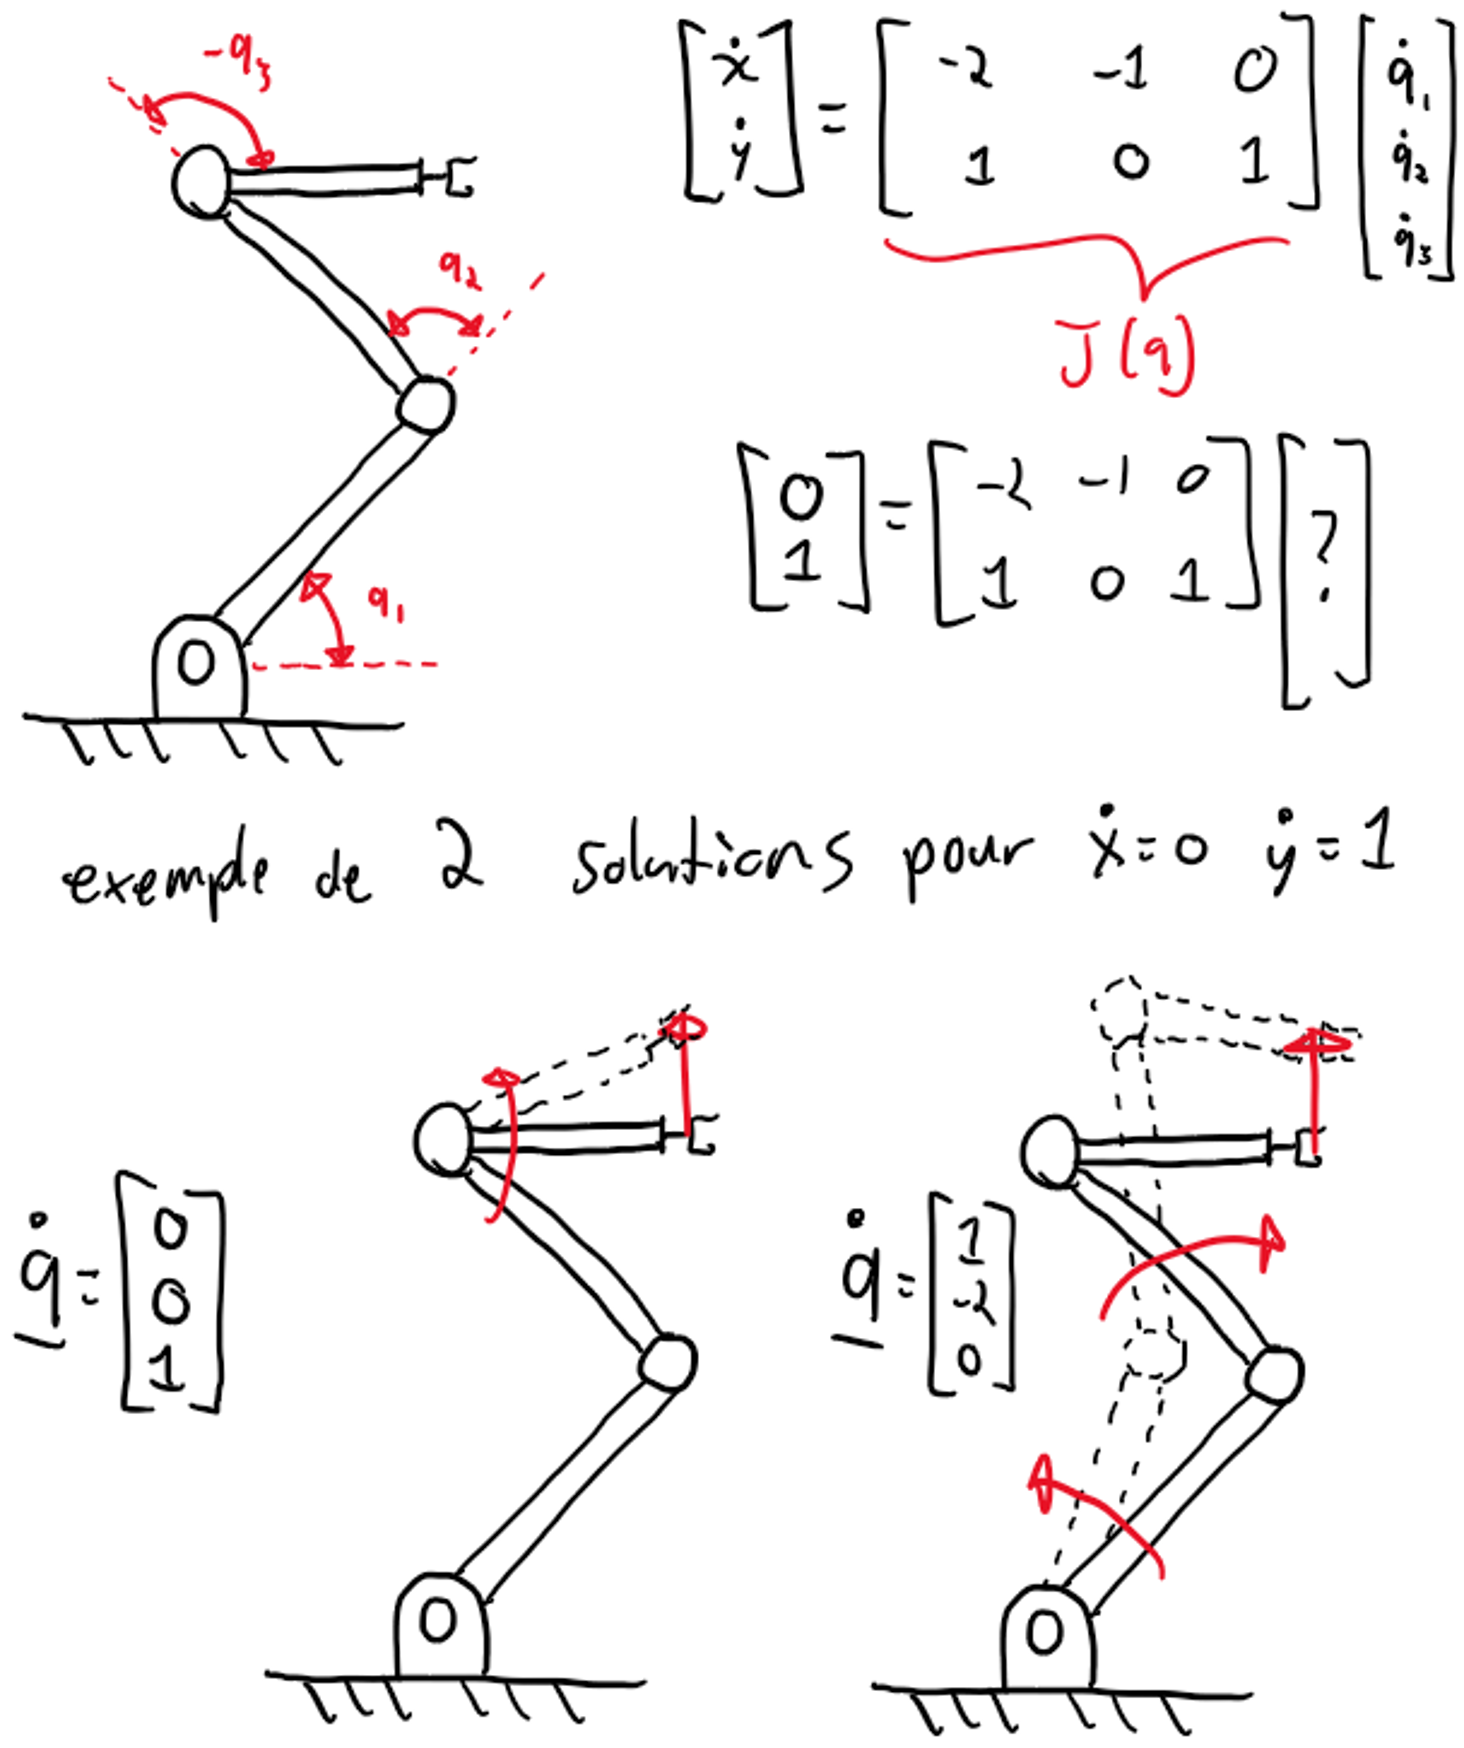
\includegraphics[width=0.45\textwidth]{robot_redo_a.png}
	\caption{Cinématique différentielle inverse d'un robot redondant ($n=3>m=2$)}
	\label{fig:robot_redo_a}
\end{figure}
%%%%%%%%%%%%%%%%%%%%%%%%%%%%%%%%%%
%
%%%%%%%%%%%%%%%%%%%%%%%%%%%%%%%%%%%
%\begin{figure}[H]
	%\centering
		%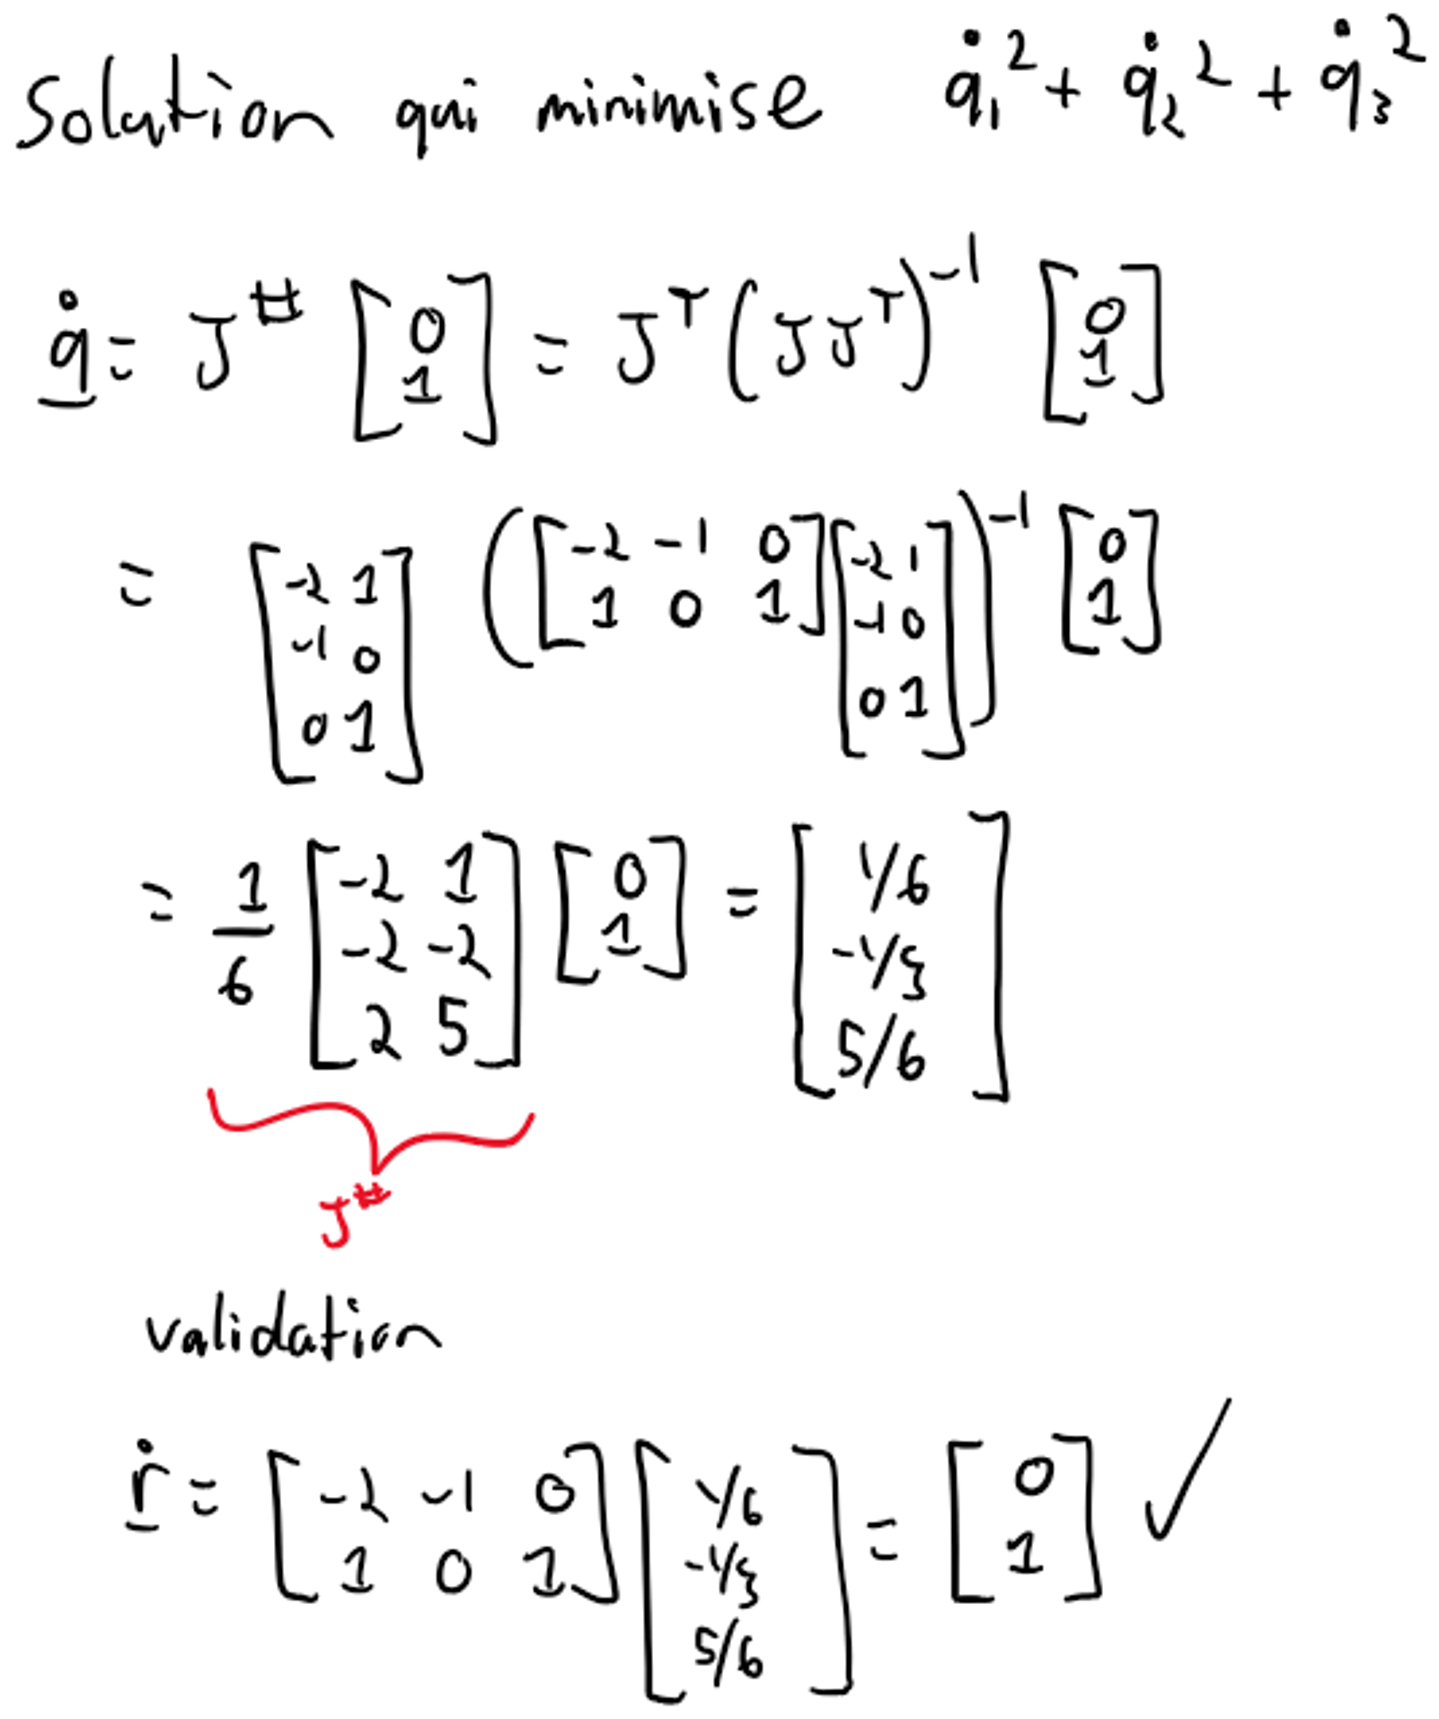
\includegraphics[width=0.55\textwidth]{robot_redo_b.png}
	%%\caption{Co-linéarité des colonnes du Jacobien pour une singularité}
	%\label{fig:robot_redo_b}
%\end{figure}
%%%%%%%%%%%%%%%%%%%%%%%%%%%%%%%%%%%
%
%%%%%%%%%%%%%%%%%%%%%%%%%%%%%%%%%%
\begin{figure}[H]
	\centering
		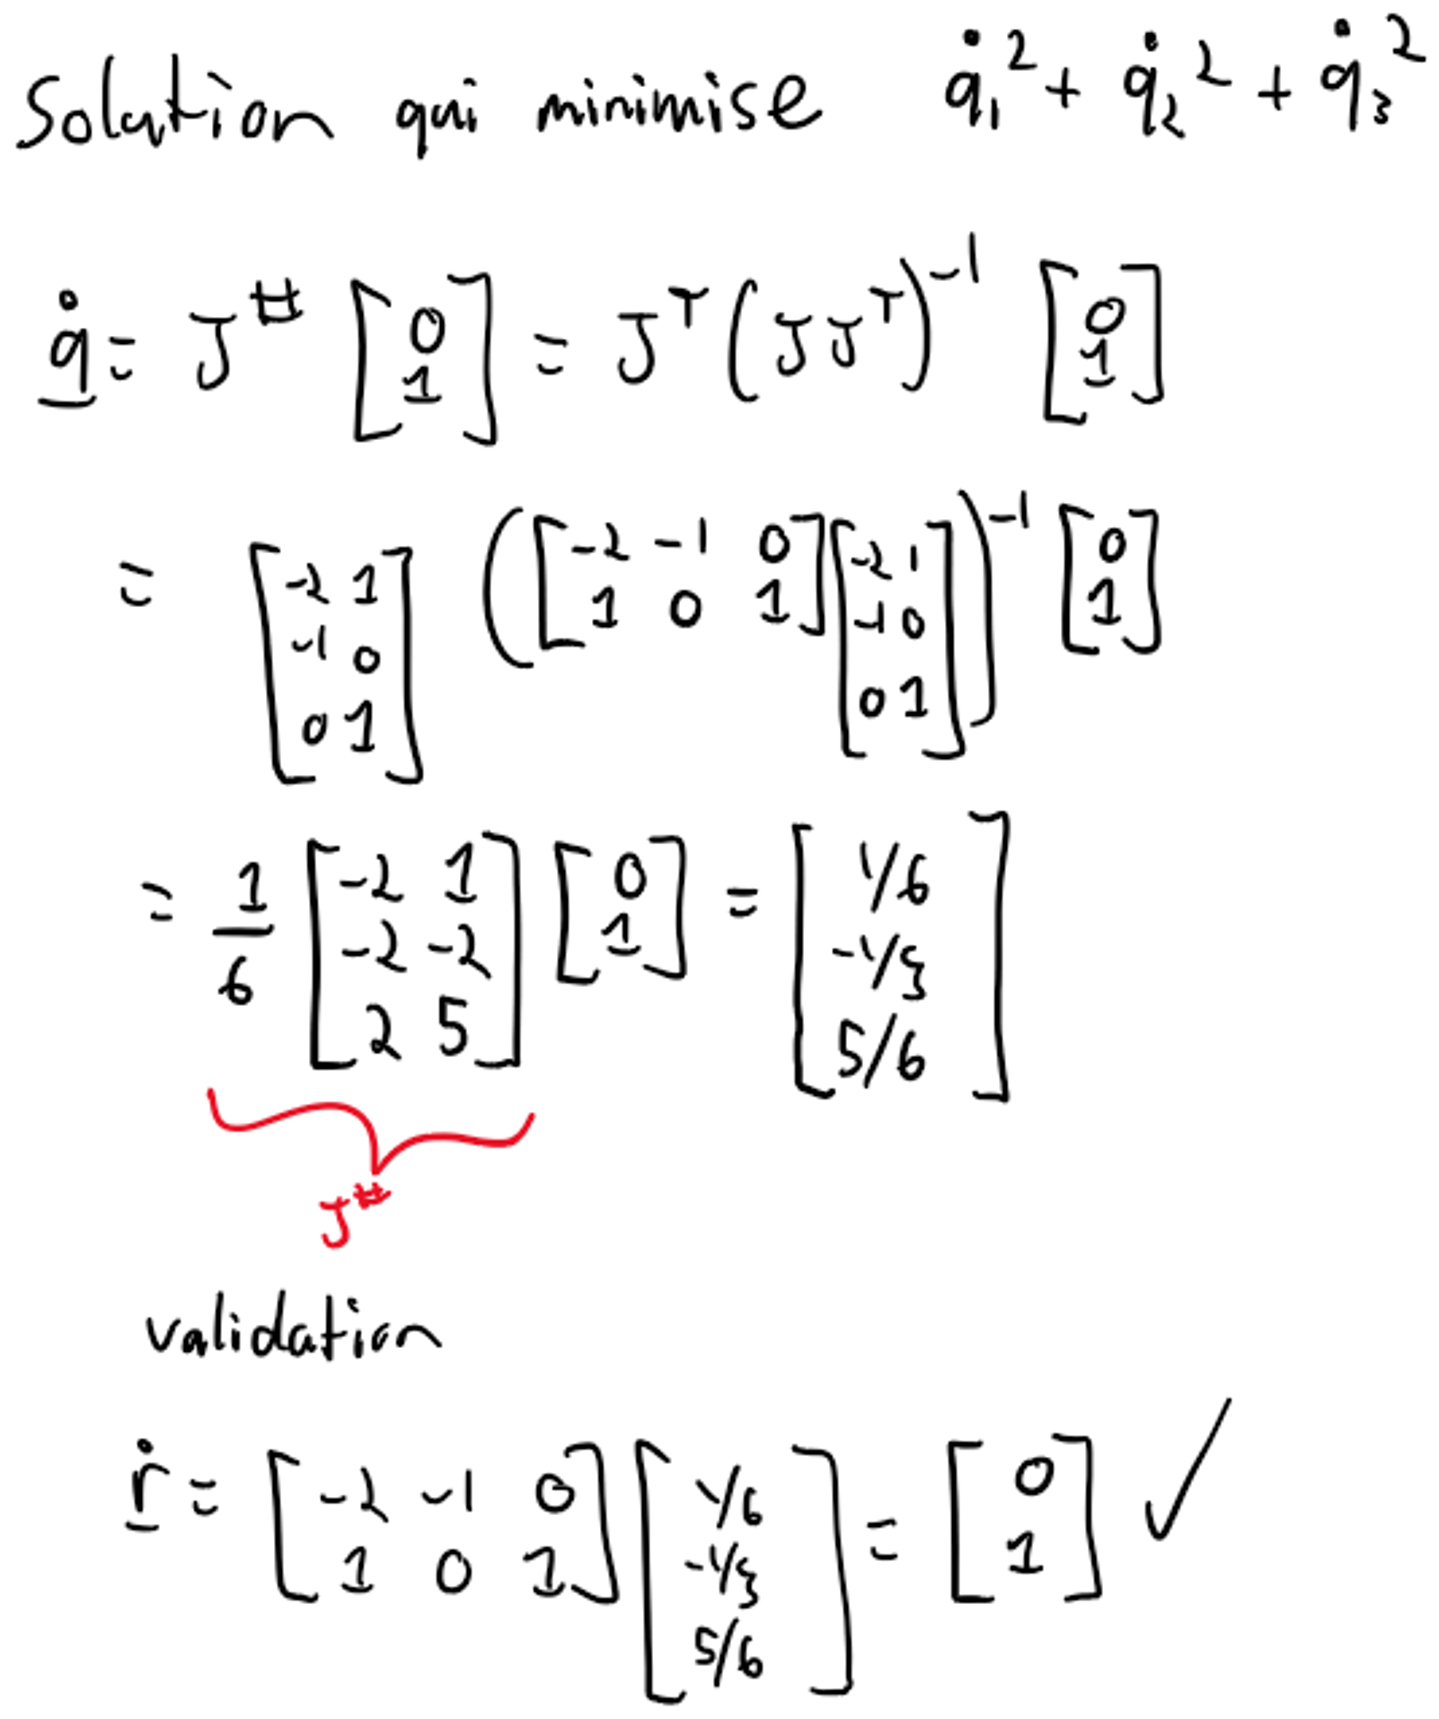
\includegraphics[width=0.45\textwidth]{robot_redo_b.png}
		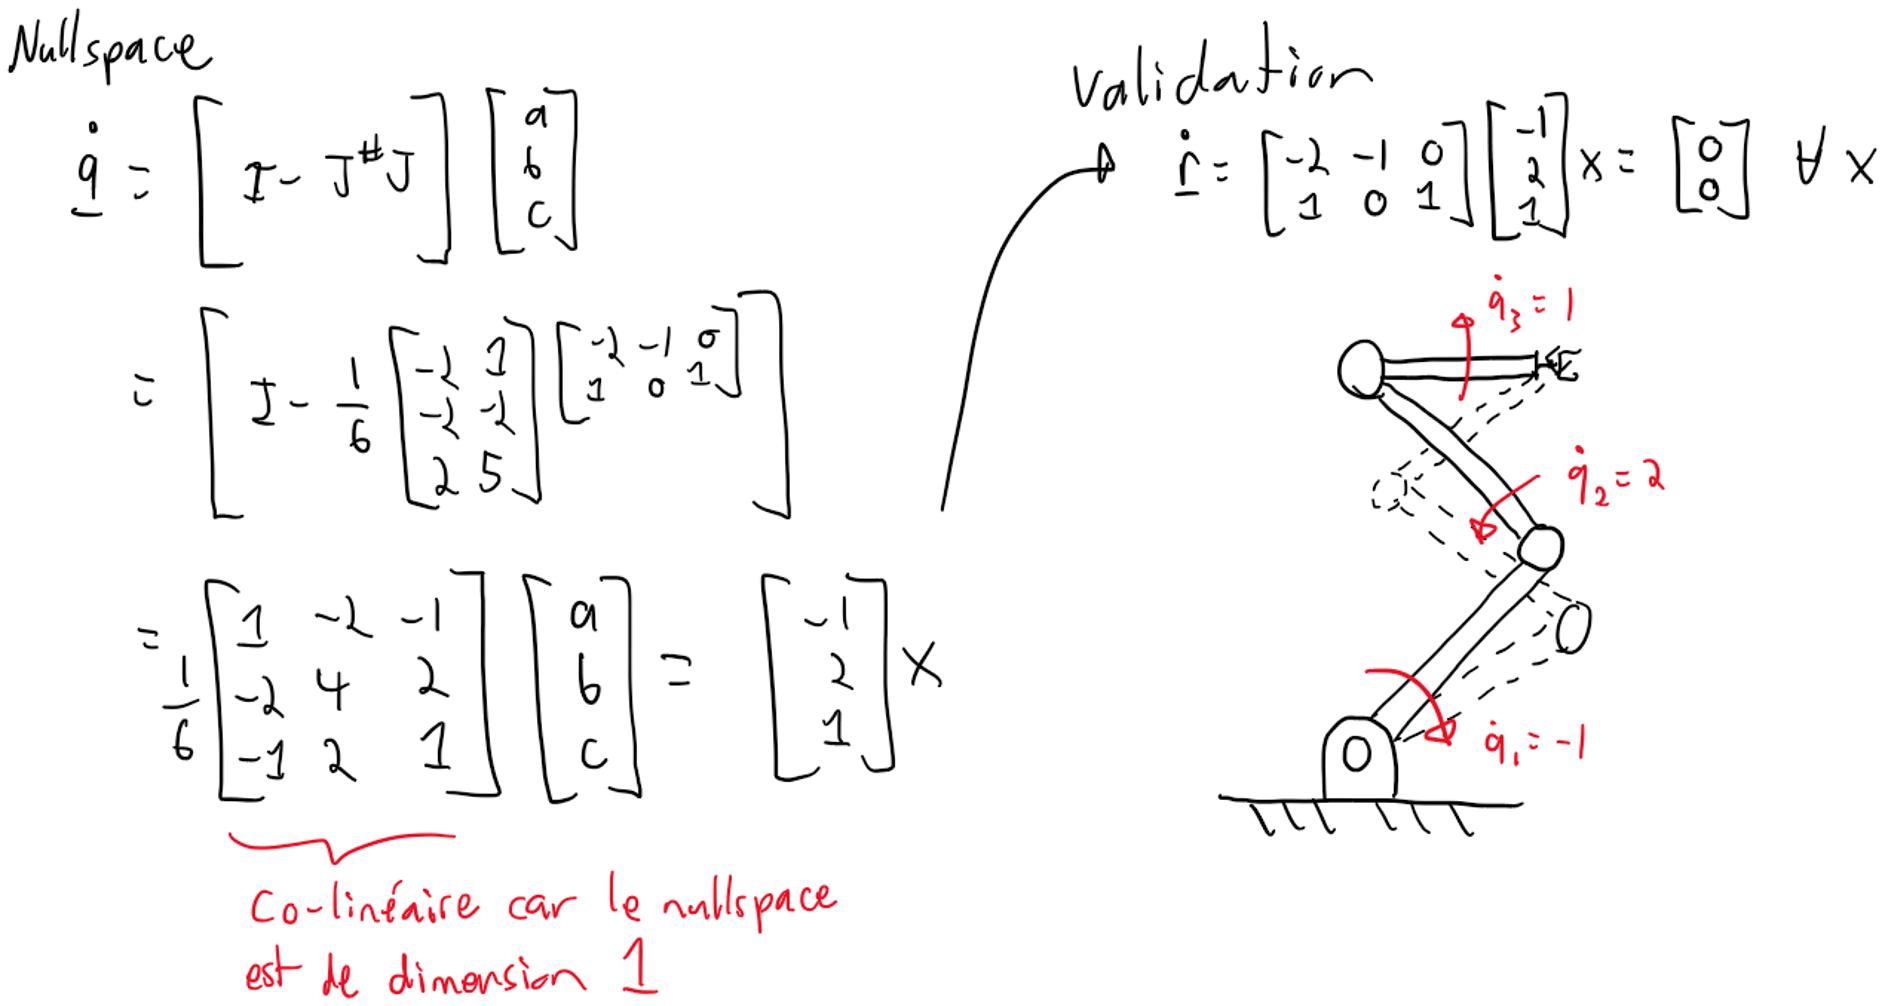
\includegraphics[width=0.85\textwidth]{robot_redo_c.png}
	\caption{Cinématique différentielle inverse d'un robot redondant: solution optimale et nullspace}
	\label{fig:robot_redo_c}
\end{figure}
%%%%%%%%%%%%%%%%%%%%%%%%%%%%%%%%%%
\end{example}





%%%%%%%%%%%%%%%%%%%%%%%%%%%%%%%%%%%%%%%%%%%%%%%%%%%%%%%%%%%%%%%%%%%%%%%%%%%%%%%%%%%%%%%%%%%%%%%%%%%%%%%%%
\subsection{Cinématique différentielle inverse pour une situation sur-contrainte}
\label{sec:overconstraintrobot}
%%%%%%%%%%%%%%%%%%%%%%%%%%%%%%%%%%

Si le nombre d'entrées $n$ est plus petit que le nombre de sorties $m$ : 
%%%%%%%%%%%%%%%%%%%%%%%%%%%%%%%%%%%
\begin{align}
n < m
\end{align} 
%%%%%%%%%%%%%%%%%%%%%%%%%%%%%%%%%%%
avec 
%%%%%%%%%%%%%%%%%%%%%%%%%%%%%%%%%%%
\begin{align}
n &= dim(\col{q}) = \quad\text{Nombre de DDL du robot} \\
m &= dim(\col{r}) = \quad\text{Coordonnées de l'espace de la tâche} 
\end{align} 
%%%%%%%%%%%%%%%%%%%%%%%%%%%%%%%%%%%
le problème de cinématique différentiel inverse est sur-contraint: il n'y a pas de solutions exactes possibles sauf pour un sous-ensemble de déplacements de l'effecteur. Le Jacobien d'une telle situation est rectangulaire, il a plus de rangées que de colonnes:
%%%%%%%%%%%%%%%%%%%%%%%%%%%%%%%%%%%
\begin{align}
\left[ \begin{array}{c}  \\ \\ \dot{\col{r}} \\ \\ \\ 
\end{array} \right]_{m \times 1}
&= 
\left[ \begin{array}{c c c} 
&&\\
&&\\
& J(\col{q}) &\\
&&\\
&&
\end{array} \right]_{m \times n}
\left[ \begin{array}{c} 
\\ \dot{\col{q}} \\ \\
\end{array} \right]_{n \times 1}
\label{eq:uoverconstraintdiffkin}
\end{align} 
%%%%%%%%%%%%%%%%%%%%%%%%%%%%%%%%%%%

Un méthode pratique pour la cinématique inverse dans ce contexte est la méthode des moindres-carré, voir la section \ref{sec:moindrecarre} pour les notions d'algèbre linéaire. L'utilisation de cette méthode permet de calculer explicitement un vecteur solution approximé $\col{\hat{\dot{q}}}$ qui minimise la norme de l'erreur entre une vitesse à l'effecteur désiré et celle obtenue avec la solution approximée. La solution au sens des moindres-carrée est calculée ainsi:
%%%%%%%%%%%%%%%%%%%%%%%%%%%%%%%%%%%
\begin{align}
\col{\hat{\dot{q}}} = \operatornamewithlimits{argmin}\limits_{\col{\dot{q}}} \left\| J \col{\dot{q}} - \col{\dot{r}} \right\|^2 = \left( J^T J\right)^{-1} J^T \, \dot{\col{r}}
\label{eq:overconstraintdiffkinleastsquare}
\end{align} 
%%%%%%%%%%%%%%%%%%%%%%%%%%%%%%%%%%%



%%%%%%%%%%%%%%%%%%%%%%%%%%%%%%%%%%%%%%%%%%%%%%%%%%%%%%%%%%%%%%%%%%%%%%%%%%%%%%%%%%%%%%%%%%%%%%%%%%%%%%%%%
\begin{example}[Exemple de cinématique différentielle inverse pour une situation sur-contrainte]
%%%%%%%%%%%%%%%%%%%%%%%%%%%%%%%%%%
\begin{figure}[H]
	\centering
		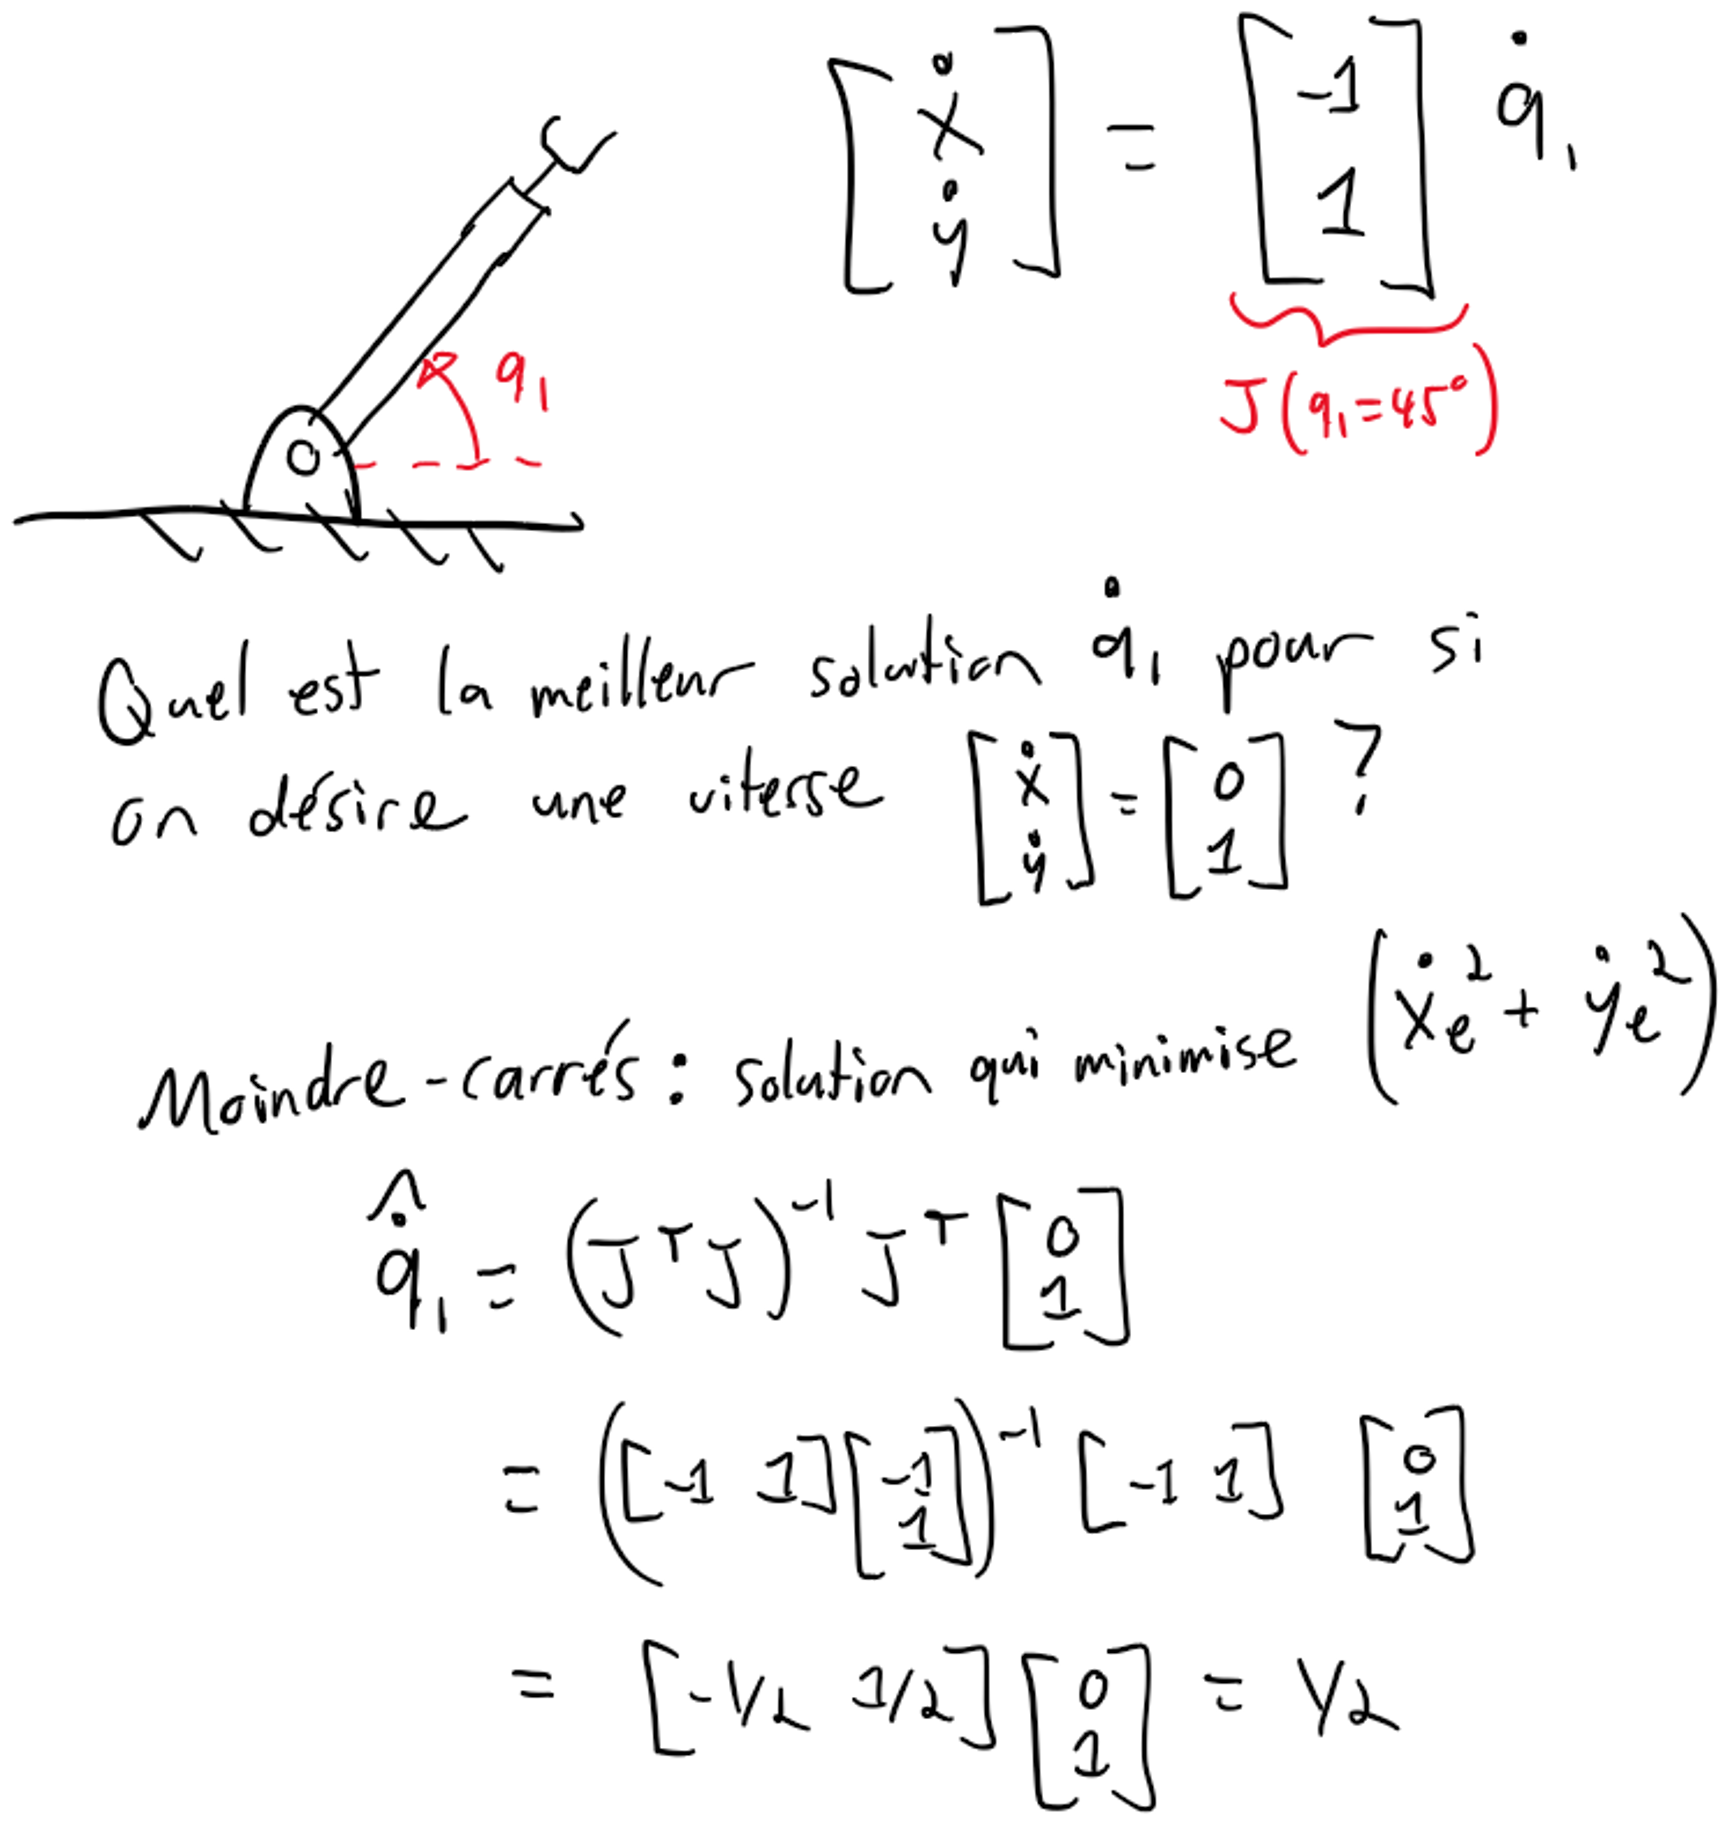
\includegraphics[width=0.55\textwidth]{robot_under.png}
	\caption{Cinématique différentielle inverse pour une situation sur-contrainte ($n=1<m=2$)}
	\label{fig:robot_under}
\end{figure}
%%%%%%%%%%%%%%%%%%%%%%%%%%%%%%%%%%
\end{example}


\newpage
%%%%%%%%%%%%%%%%%%%%%%%%%%%%%%%%%%%%%%%%%%%%%%%%%%%%%%%%%%%%%%%
\section{Manipulabilité d'un robot manipulateur}
\label{sec:velocitymanipulability}

Lorsqu'on désire effectuer une tâche avec l'effecteur d'un robot à une certaine position, la première question est: est-ce que le robot est capable d'atteindre cette position, i.e. est-ce que la position cible est dans l'espace de travail? Si la position est atteignable, une deuxième question doit être posée: est-ce que le robot est capable de bouger arbitrairement à cette position? Cette deuxième question est la notion de manipulabilité du robot manipulateur. 

Comme discuté à la section \ref{sec:singu}, lorsque le robot est à une configuration singulière l'effecteur est incapable de bouger dans certaines directions. On considère donc que la manipulabilité d'un robot n'est pas bonne sur une singularité. Toutefois, il est utile d'avoir une notion non-binaire de la manipulabilité, car même si un robot n'est pas parfaitement sur une singularité, certaines configurations peuvent nécessiter de très grandes vitesses aux joints pour satisfaire des vitesses cartésiennes de l'effecteur. Donc en considérant les limites de vitesse des joints le robot est en fait incapable d'executer certain vecteur vitesse à son effecteur proche d'une singularité. Les indices de manipulabilité sont des fonctions scalaires qui ont comme objectif de caractériser si un robot dans une certaine configuration est proche d'une singularité.  Ces indicateurs peuvent être utile lorsque qu'on conçoit la cinématique d'un robot ou lorsque qu'on programme des tâches avec un robot existant.


\subsubsection{Indices de manipulabilité d'un robot manipulateur}

Pour les situations ou la matrice jacobienne $J$ du robot est carré, le déterminant est un bon indice de la manipulabilité du robot:
%%%%%%%%%%%%%%%%%%%%%%%%%%%%%%%%%%%
\begin{align}
m_1(\col{q})= det( J(\col{q}) )
\end{align} 
%%%%%%%%%%%%%%%%%%%%%%%%%%%%%%%%%%%
Le déterminant correspond au volume du prisme généré par les colonnes du jacobien qui correspondent à des vecteurs vitesses de l'effecteur pour des vitesses de joints unitaires de chacun des axes:
%%%%%%%%%%%%%%%%%%%%%%%%%%%%%%%%%%
\begin{figure}[H]
	\centering
		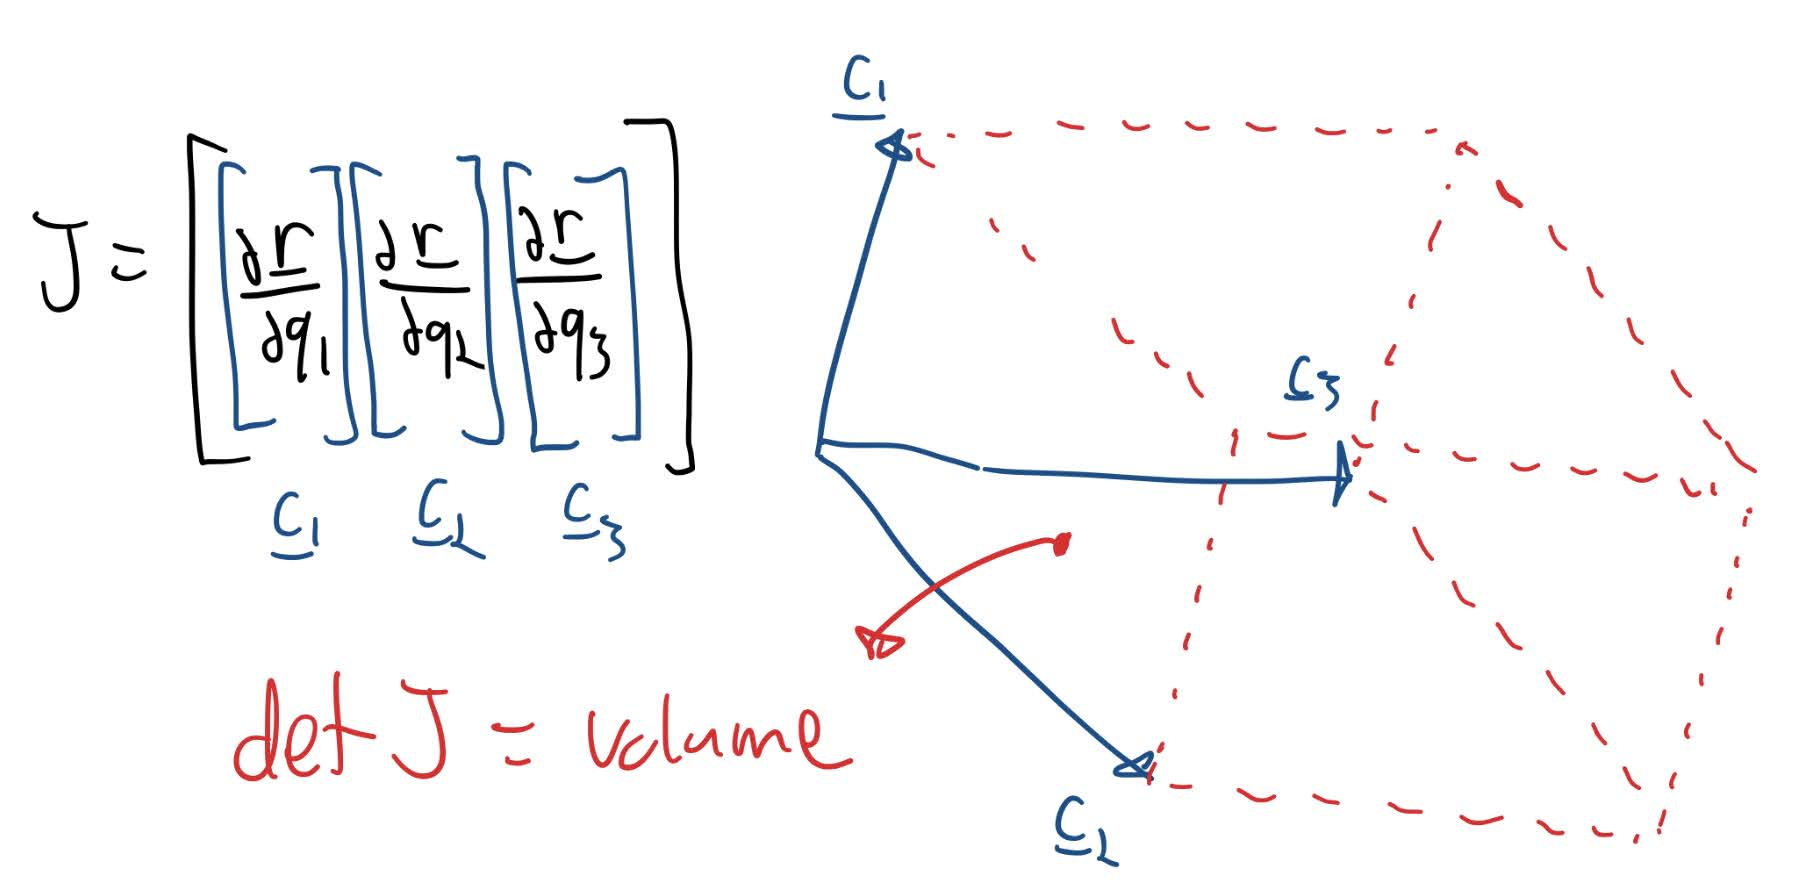
\includegraphics[width=0.75\textwidth]{fig/jacobianvolume.jpg}
	\caption{Volume de la matrice jacobienne}
	\label{fig:jacobianvolume}
\end{figure}
%%%%%%%%%%%%%%%%%%%%%%%%%%%%%%%%%%
Dès que un des vecteurs est très petit, ou bien quand les vecteurs sont colinéaires, le volume du prisme devient très petit ce qui correspond à une mauvaise manipulabilité.


Un autre indicateur souvent utilisé est les valeurs singulières de la matrice jacobienne. Les valeurs singulières $\mu$ sont relié aux valeurs propres $\lambda$ du produit $J^TJ$
%%%%%%%%%%%%%%%%%%%%%%%%%%%%%%%%%%%
\begin{align}
\mu^2_{i}( J(\col{q}) ) = \lambda_i( J(\col{q})^T J(\col{q}) )
\end{align} 
%%%%%%%%%%%%%%%%%%%%%%%%%%%%%%%%%%%
Pour relié à un indice de manipulabilité, on peut surveillez la plus petite valeur singulière ou bien le ratio entre la plus petite et la plus grande:
%%%%%%%%%%%%%%%%%%%%%%%%%%%%%%%%%%%
\begin{align}
m_2(\col{q})= \mu_{min}( J(\col{q}) ) \\
m_3(\col{q})= \frac{\mu_{min}( J(\col{q}) ) }{\mu_{max}( J(\col{q}) ) }\\
\end{align} 
%%%%%%%%%%%%%%%%%%%%%%%%%%%%%%%%%%%
La valeur $\mu_{min}$ correspond à la norme minimal du vecteur vitesse de l'effecteur produit par un vecteur de vitesse aux joints unitaire.


\subsubsection{Ellipsoïde de vitesse}

%%%%%%%%%%%%%%%%%%%%%%%%%%%%%%%%%%
\begin{figure}[htb]
	\centering
		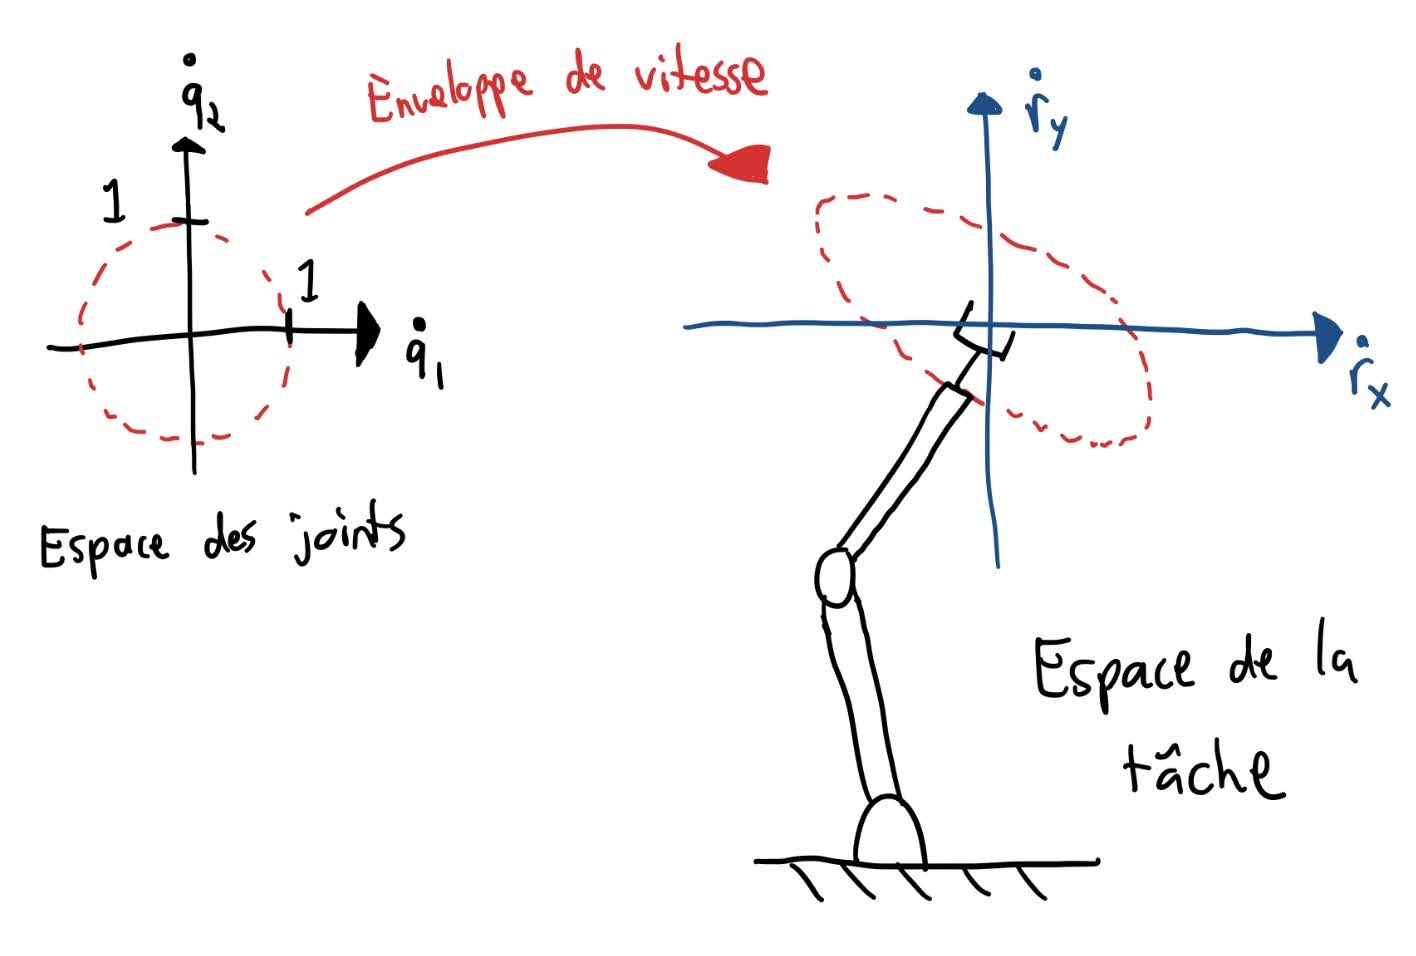
\includegraphics[width=0.85\textwidth]{fig/velocitymanipulabilityellipsoid.jpg}
	\caption{Ellipsoïde de vitesse}
	\label{fig:manipulabilityellipsoid}
\end{figure}
%%%%%%%%%%%%%%%%%%%%%%%%%%%%%%%%%%

L'ellipsoïde de vitesse d'un robot manipulateur est l'enveloppe des vecteurs vitesses possibles à l'effecteur pour des vecteurs de vitesse des joints unitaires, voir \ref{fig:manipulabilityellipsoid}. L'enveloppe de vitesses possibles à l'effecteur, résultant d'un vecteur de vitesse des joints unitaire, peut être calculer en débutant avec une équation qui contraint la norme du vecteur de la vitesse des joint et en substituant $\dot{\col{q}}$ par $J^{-1} \dot{\col{r}}$ dans l'équation:
%%%%%%%%%%%%%%%%%%%%%%%%%%%%%%%%%%%
\begin{align}
1 &= \dot{\col{q}}^T \dot{\col{q}} \\
1 &= \dot{\col{r}}^T J^{-T} J^{-1} \dot{\col{r}} \\
1 &= \dot{\col{r}}^T (J J^T)^{-1} \dot{\col{r}} \\
1 &= \dot{\col{r}}^T A^{-1} \dot{\col{r}} \quad\quad \text{avec} \quad\quad A = J J^T
\end{align} 
%%%%%%%%%%%%%%%%%%%%%%%%%%%%%%%%%%%
On obtient donc une équation quadratique pour laquelle l'ensemble des solutions possibles forment une ellipse. Les axes principaux de l'ellipse correspondent aux valeurs propres et vecteurs propres de la matrice $J J^T$. 

%%%%%%%%%%%%%%%%%%%%%%%%%%%%%%%%%%
\begin{figure}[H]
	\centering
		%\includegraphics[width=0.85\textwidth]{}
	\caption{TODO: ellipse 3D}
	%\label{fig:manipulabilityellipsoid}
\end{figure}
%%%%%%%%%%%%%%%%%%%%%%%%%%%%%%%%%%

Un lien peu aussi être fait directement avec les valeurs singulière de la matrice $J$. Détails à venir!

\begin{example}[Indice de manipulabilité pour un robot à 2 DDL]

Une exemple simple pour illustré l'indice de manipulabilité est un robot planaire à 2 DDL comme illutré à la Figure \ref{fig:2dof_manip_graph}, pour lequel on peut analyser la manipulabilité pour divers position de l'effecteur sur l'axe horizontal. La manipulabilité est nulle lorsque le coude est complètement plié (le robot est sur une singularité et ne peut bouger horizontalement), nulle lorsque le coude est complètement déplié (le robot est sur une singularité de ne peut bouger horizontalement) et optimale entre les deux lorsque le coude est partielement plié.

%%%%%%%%%%%%%%%%%%%%%%%%%%%%%%%%%%
\begin{figure}[H]
	\centering
		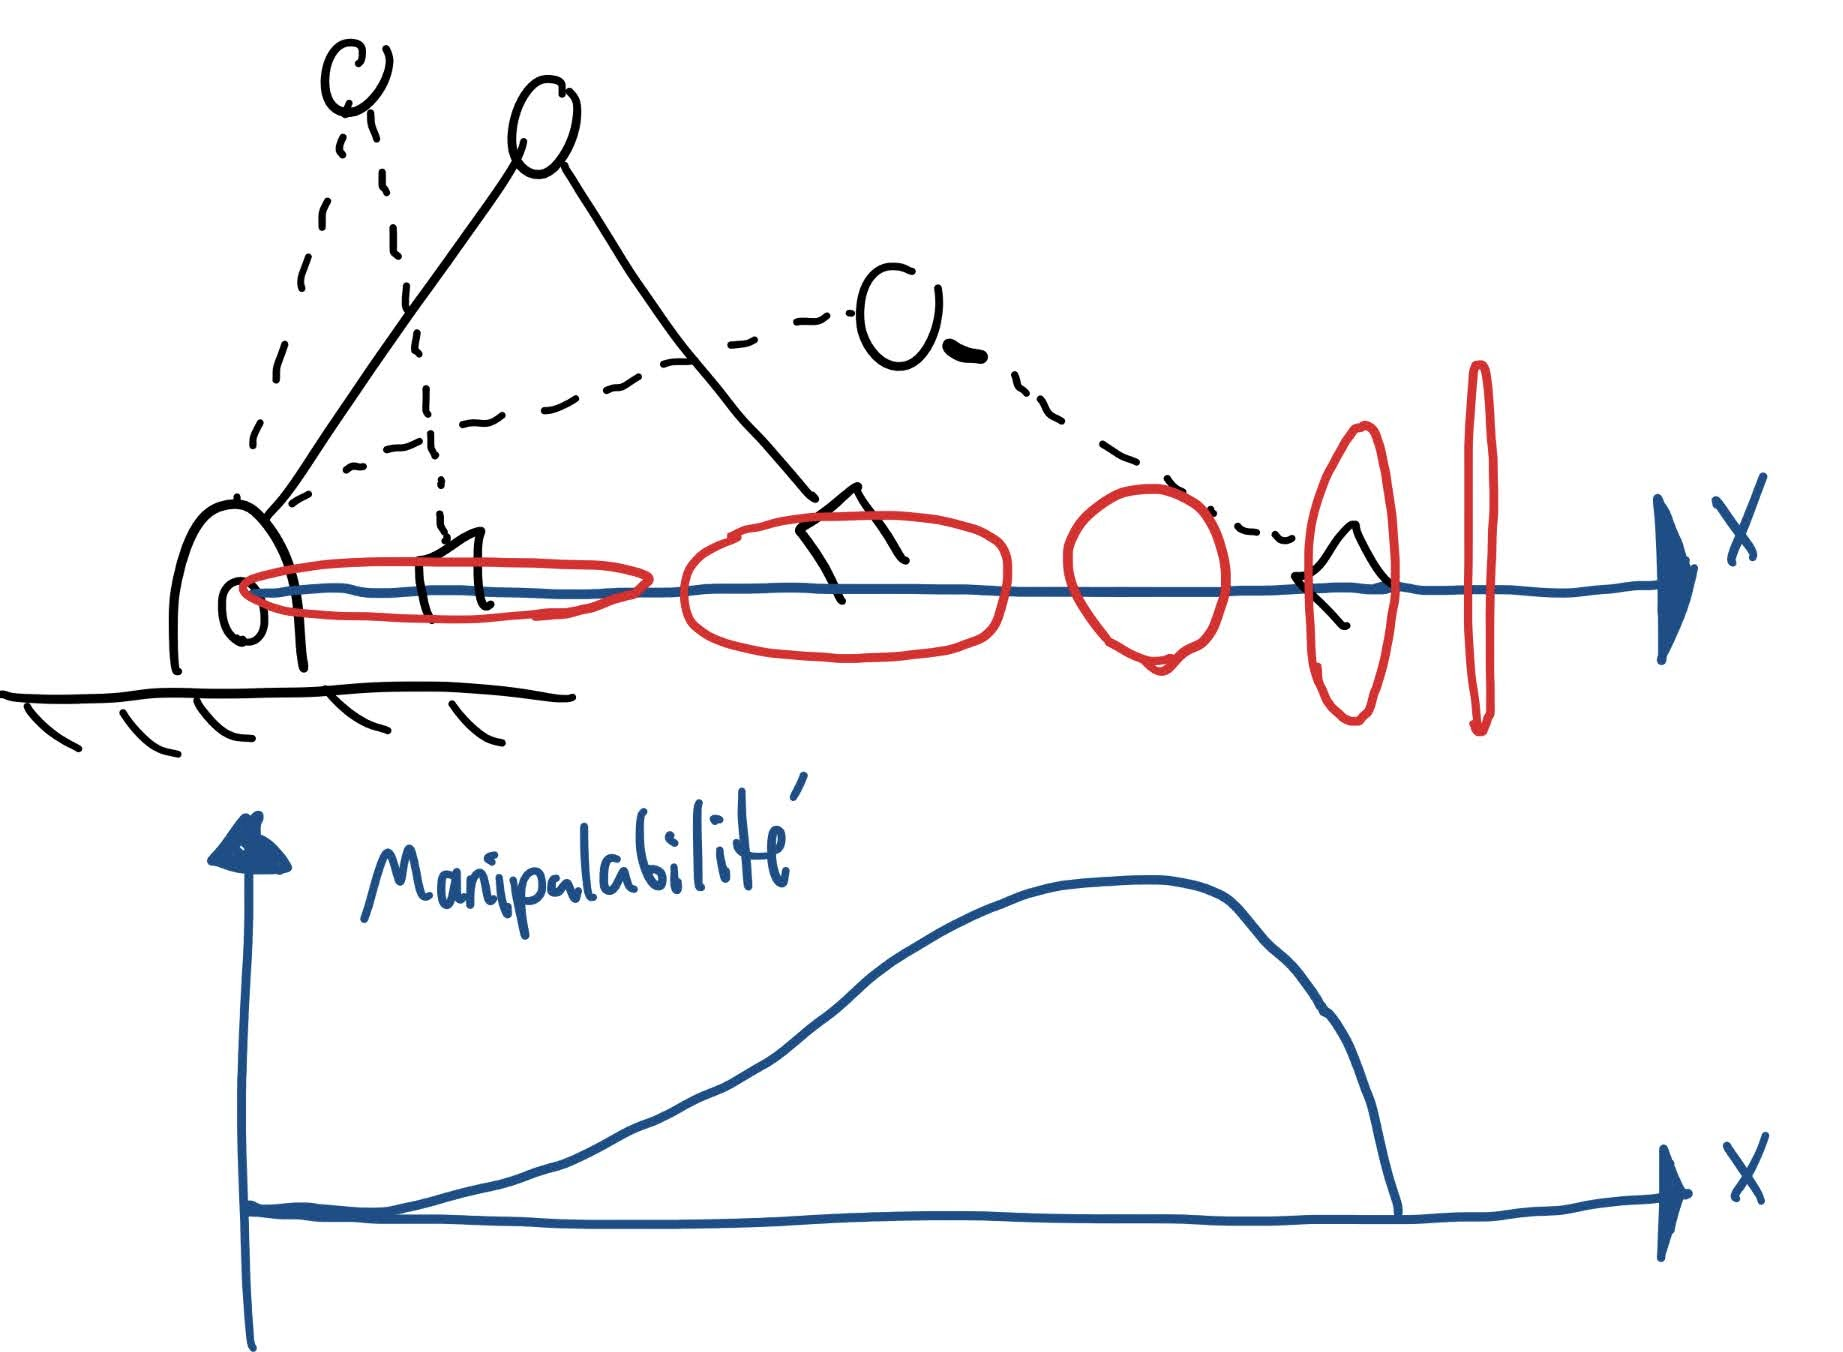
\includegraphics[width=0.65\textwidth]{fig/2dof_manip_graph.jpg}
	\caption{Exemple de l'indice de manipulabilité pour un robot à 2 DDL}
	\label{fig:2dof_manip_graph}
\end{figure}
%%%%%%%%%%%%%%%%%%%%%%%%%%%%%%%%%%

\end{example}







\newpage
%%%%%%%%%%%%%%%%%%%%%%%%%%%%%%%%%%%%%%%%%%%%%%%%%%%%%%%%%%%%%%%
\section{Relation entre les variables d'accélération}
\label{sec:accjointspace}


Pour faire le lien en l'accélération dans l'espace des joints et l'accélération dans l'espace de la tâche, il suffit de dériver par rapport au temps l'expression de la cinématique différentielle, autrement dit on dérive deux fois par rapport au temps l'équation de la cinématique directe:
%%%%%%%%%%%%%%%%
\begin{align}
\text{Cinématique directe:}  \quad \col{r} &= f\left( \, \col{q} \, \right) \\
\text{Cinématique différentielle:} \quad \col{\dot{r}} &= J\left( \, \col{q} \, \right) \, \col{\dot{q}} \\
\text{Cinématique différentielle ordre-2:} \quad \col{\ddot{r}} &= J\left( \, \col{q} \, \right) \, \col{\ddot{q}}  + \dot{J} \left( \, \col{q}  , \col{\dot{q}} \, \right) \, \col{\dot{q}} 
\label{eq:ddj}
\end{align}
%%%%%%%%%%%%%%%
Comme on dérive un produit avec deux termes qui varient dans le temps, l'accélération $\col{\ddot{r}}$ est le résultat de deux effets représentés par deux termes. Le premier terme est simplement l'accélération des joints fois le Jacobien, i.e. les bras de leviers. Le deuxième terme est une contribution à l'accélération de l'effecteur qui vient de la variation temporelle du Jacobien. Comme le Jacobien a seulement une dépendance directe aux positions $\col{q}$, on peut exprimer son taux de variation temporelle comme sa dérivée par rapport à $\col{q}$ fois le vecteur-colonne de vitesse $\col{\dot{q}}$, selon le principe de dérivée en chaînes:
%%%%%%%%%%%%%%%%
\begin{align}
\dot{J} = \frac{ \partial J}{\partial \col{q}} \, \col{\dot{q}} 
\end{align}
%%%%%%%%%%%%%%%
Toutefois ici, on dérive une matrice $m \times n$ par un vecteur-colonne $n \times 1$, le résultat est donc un tenseur (ses composantes si on veux être rigoureux) d'ordre 3, i.e. une matrice 3D $m \times n \times n$ :
%%%%%%%%%%%%%%%%%%%%
\begin{align}
%%%%%%%%%%%%%%%%%%%%
\left[ \begin{array}{c}  \\ \dot{J} \\ \\
\end{array} \right]_{m \times n}
&= 
\underbrace{
\left[ \begin{array}{c c c} 
&&\\
& \frac{ \partial J}{\partial \col{q}} &\\
&&
\end{array} \right]_{m \times n \times n}}_{\text{Tenseur d'ordre 3
%\footnote{Techniquement c'est les composantes du tenseur qui sont contenue dans une "matrice" à 3 dimensions.}
}}
\left[ \begin{array}{c} 
\\ \col{\dot{q}} \\ \\
\end{array} \right]_{n \times 1}
%%%%%%%%%%%%%%%%%%%%
\label{eq:jdot}
\end{align}
%%%%%%%%%%%%%%%
Lorsqu'on travail avec des tenseurs d'ordre 3 et plus, il est normalement plus facile de travailler avec des équations qui relient les composantes avec une notation indicielle. La composante $ijk$ du tenseur qui résultent de la dérivation du Jacobien $J$ par $\col{q}$ est égale à la dérivée de l'élément $ij$ du Jacobien par rapport à l'élément $k$ du vecteur-colonne $\col{q}$:
%%%%%%%%%%%%%%%%
\begin{align}
\left[\frac{ \partial J}{\partial \col{q}} \right]_{ijk} = \frac{ \partial J_{ij} }{\partial q_k } 
\end{align}
%%%%%%%%%%%%%%%
 Donc le produit intérieur exprimé à l'équation \eqref{eq:jdot} peut être exprimé directement comme une sommation à effectuer pour calculer l'élément $ij$ de la matrice $\dot{J}$:
%%%%%%%%%%%%%%%%
\begin{align}
\dot{J}_{ij} = \sum_k \left( \frac{ \partial J_{ij} }{\partial q_k } \dot{q}_k \right)
\end{align}
%%%%%%%%%%%%%%%
Finalement, il est possible d'exprimer directement l'équation \eqref{eq:ddj} en termes de composantes, d'indices et de sommations:
%%%%%%%%%%%%%%%%
\begin{align}
\ddot{r}_{i} =  
\sum_j J_{ij} \ddot{q}_j
+
\sum_j 
\sum_k  \frac{ \partial J_{ij} }{\partial q_k } \dot{q}_k 
\dot{q}_j
\end{align}
%%%%%%%%%%%%%%%
Plus de détails sur les équivalences entre les opérations en termes de matrices/vecteur-colonnes/tenseurs et les opérations en termes de composantes et d'indices sont disponibles à la section \ref{sec:vectoropindex}.




\newpage
\section{Résumé du chapitre}


Vecteur vitesse et dérivée d'un vecteur position (base $b$ non-inertielle)
%%%%%%%%%%%%%%%%
\begin{align}
\underbrace{
\vec{v}_{B} = {}^{b}\frac{d}{dt} \vec{r}_{B/A} +  \vec{w}_{b/a} \, \times \, \vec{r}_{B/A}
}_{\text{Relation vectorielle}}
\quad \Leftrightarrow \quad 
\underbrace{
\col{v}_{B}^{a} = {}^{a}R^b \left[ \col{\dot{r}}^b_{B/A} +  (\col{w}_{b/a}^b)^{\times} \col{r}^b_{B/A}  \right] 
}_{\text{Relation matricielle des composantes}}
\end{align}
%%%%%%%%%%%%%%%

Vecteur accélération et dérivée seconde d'un vecteur position
%%%%%%%%%%%%%%%%
\begin{align}
\vec{a}_{B} = 
{}^{b}\frac{d^2}{dt^2} \vec{r}_{B/A} 
+  
{}^{b}\frac{d}{dt} \vec{w}_{b/a} \, \times \, \vec{r}_{B/A}
+
\underbrace{
2 \vec{w}_{b/a} \, \times \, {}^{b}\frac{d^2}{dt^2} \vec{r}_{B/A}
}_{\text{Coriolis}}
+
\underbrace{
\vec{w}_{b/a} \, \times \vec{w}_{b/a} \, \times \,
\vec{r}_{B/A}
}_{\text{Centrifuge}}
\end{align}
%%%%%%%%%%%%%%%

%%%%%%%%%%%%%%%%
\begin{align}
\col{a}_{B}^{a} 
= 
{}^{a}R^b \left[ 
\col{\ddot{r}}^b_{B/A}
+ 
(\col{\dot{w}}_{b/a}^b)^{\times} \col{r}^b_{B/A}  
+
\underbrace{
2 (\col{w}_{b/a}^b)^{\times} \col{\dot{r}}^b_{B/A}  
}_{\text{Coriolis}}
+
\underbrace{
(\col{w}_{b/a}^b)^{\times} (\col{w}_{b/a}^b)^{\times} \col{r}^b_{B/A}  
}_{\text{Centrifuge}}
\right] 
\end{align}
%%%%%%%%%%%%%%%

Dérivée temporelle d'une matrice de rotation:
%%%%%%%%%%%%%%%%
\begin{equation}
\dot{R} = \frac{d}{dt} R = (\col{w})^x \, R
\end{equation}
%%%%%%%%%%%%%%%
%%%%%%%%%%%%%%%%
\begin{equation}
{}^{a}\dot{R}^b =  (\col{w}_{b/a}^a)^{\times} \, {}^{a}R^b =   {}^{a}R^b \, (\col{w}_{b/a}^b)^{\times}
\end{equation}
%%%%%%%%%%%%%%%

Relations différentielles entre l'espace des joints et de la tâche:
%%%%%%%%%%%%%%%%
\begin{align}
\col{r} &= f\left( \, \col{q} \, \right) \\
\col{\dot{r}} &= J\left( \, \col{q} \, \right) \, \col{\dot{q}} \\
\col{\ddot{r}} &= J\left( \, \col{q} \, \right) \, \col{\ddot{q}}  + \dot{J} \left( \, \col{q}  , \col{\dot{q}} \, \right) \, \col{\dot{q}} 
\end{align}
%%%%%%%%%%%%%%%

La matrice Jacobienne:
%%%%%%%%%%%%%%%%
\begin{equation}
J\left( \col{q} \right) = \frac{\partial \col{r}}{\partial \col{q}} = 
\left[ \begin{array}{c c c} 
\frac{\partial r_1 }{\partial q_1}   &  \hdots & \frac{\partial r_1 }{\partial q_n} \\ 
\vdots                               &  \ddots & \vdots                             \\
\frac{\partial r_m }{\partial q_1}   &  \hdots & \frac{\partial r_m }{\partial q_n}
\end{array} \right]_{m \times n}
\end{equation}
%%%%%%%%%%%%%%%%